\documentclass[11pt,a4paper]{article}

\usepackage[T1]{fontenc}
\usepackage[utf8]{inputenc}
\usepackage[english]{babel}
\usepackage[a4paper,margin=0.72in]{geometry}
\usepackage{parskip}
\usepackage{graphicx}
\usepackage{booktabs}
\usepackage{tabularx}
\usepackage{array}
\usepackage{longtable}
\usepackage{float}
\usepackage{xcolor}
\usepackage[colorlinks=true,linkcolor=blue!55!black,urlcolor=blue!55!black]{hyperref}

\setlength{\parindent}{0pt}
\setlength{\parskip}{0.55em}
\emergencystretch=1.5em

\newcommand{\figref}[1]{Figure~\ref{#1}}
\newcommand{\tabref}[1]{Table~\ref{#1}}
\newcommand{\appendixfig}[3]{%
\begin{figure}[H]
\centering
\includegraphics[width=#1\textwidth]{#2}
\caption{#3}
\end{figure}
}

\title{\textbf{DSA210 Term Project Final Report}\\
\large Entertainment Behavior Under Academic Pressure}
\author{
Nihat Omer Karaca\\
\texttt{omer.karaca@sabanciuniv.edu}\\
\texttt{nihatomer.karaca@gmail.com}
}
\date{}

\begin{document}

\maketitle

\begin{abstract}
This project analyzes my entertainment behavior across YouTube, Spotify, Netflix, Prime Video, and academic calendar periods. The goal is to understand whether daily entertainment activity changes under academic pressure and whether daily platform behavior can be used to classify ordinary term, final exam, and summer work periods. The project includes public-data preparation, exploratory data analysis, hypothesis testing, machine learning, and a public website for presentation.
\end{abstract}

\tableofcontents
\newpage

\section{Motivation}

The motivation for this project came from a practical question about my own daily life: what am I doing daily other than what I am supposed to do? I decided to explore my entertainment behavior because it could provide part of the answer. Instead of keeping this as an intuition, I wanted to test it with data from the platforms I actually use.

At the beginning, I considered several personal data exports, including ChatGPT, Instagram, Netflix, Spotify, Twitter, and YouTube. After evaluating the scope and privacy risks, I excluded Instagram and Twitter because they would increase the complexity too much for this version. I also did not use ChatGPT because it is a different behavioral domain and would require heavier privacy and text-processing decisions. The final project focuses on YouTube, Spotify, Netflix, Prime Video, and the academic calendar, which also represents a significant part of my daily life.

The project is intentionally entertainment-focused. YouTube represents short-form and mixed video activity, Spotify represents music listening duration, and Netflix plus Prime Video represent long-form streaming. The academic calendar is used as the label source for academic periods, not as a behavioral dataset.

\section{Data Source}

The data comes from personal platform exports and the Sabanci University academic calendar. Private raw exports were processed locally, and only public, reduced, analysis-ready files are kept in the repository under \texttt{data\_github/}. Private identifiers, local source paths, and unnecessary account-level fields were removed or masked before publication.

\begin{table}[H]
\centering
\small
\caption{Prepared public datasets used in the analysis.}
\label{tab:datasets}
\begin{tabularx}{\textwidth}{l r l X}
\toprule
\textbf{Dataset} & \textbf{Rows} & \textbf{Date range} & \textbf{Role in analysis}\\
\midrule
YouTube & 34,317 activity rows & 2022-04-17 to 2026-03-15 & Watch/search-style video behavior with timestamps.\\
Spotify & 178,202 streaming rows & 2019-07-27 to 2026-03-14 & Music listening behavior with timestamps and listening duration.\\
Netflix & 2,493 viewing rows & 2020-02-25 to 2026-03-10 & Long-form viewing history with visible titles.\\
Prime Video & 719 watch rows & 2022-03-30 to 2026-03-19 & Long-form viewing parsed into movie and episode records.\\
Academic calendar & Calendar labels & 2021--2022 to 2025--2026 & Label source for ordinary term, final exam, and summer work periods.\\
\bottomrule
\end{tabularx}
\end{table}

The common comparison window is 2022-04-17 to 2026-03-10. This is the date range where all four entertainment datasets overlap. After daily aggregation, the combined panel contains 1,424 daily rows. If a platform had no row on a date, it was treated as zero activity for that platform after aggregation.

\section{Data Analysis}

The analysis had five main stages: data cleaning, exploratory data analysis, hypothesis testing, machine learning, and public presentation through the website as an additional way to show my findings and what I did.

\subsection{Data Cleaning and Preparation}

Each platform had a different export structure. Spotify was already structured and duration-based. YouTube required activity normalization, timestamp handling, action categorization, and masking. Netflix was simpler but mostly date-level. Prime Video required parsing into movie and episode records.

After platform-specific cleaning, each dataset was converted into a common date structure using \texttt{fine\_date}. YouTube and Spotify timestamps were also used to create late-evening variables, especially after-21:30 activity. The platform-level daily features were then merged with the academic calendar labels into one combined daily panel.

The main daily features include YouTube watched/search counts, YouTube after-21:30 count, Spotify hours, Spotify stream count, Spotify unique tracks, Spotify after-21:30 hours, Netflix count, Prime Video count, Netflix plus Prime count, and the number of distinct active entertainment platforms per day.

\subsection{Exploratory Data Analysis}

The EDA was performed in two layers. First, I inspected each platform separately to understand the structure and timing of the data. Second, I created combined daily plots to compare platforms and academic periods.

\figref{fig:coverage} shows the dataset coverage and explains why a common date window was needed. \figref{fig:active-days} shows that the platforms have very different activity densities. Spotify appears on many more days, while Netflix and Prime Video are much sparser.

\begin{figure}[H]
\centering
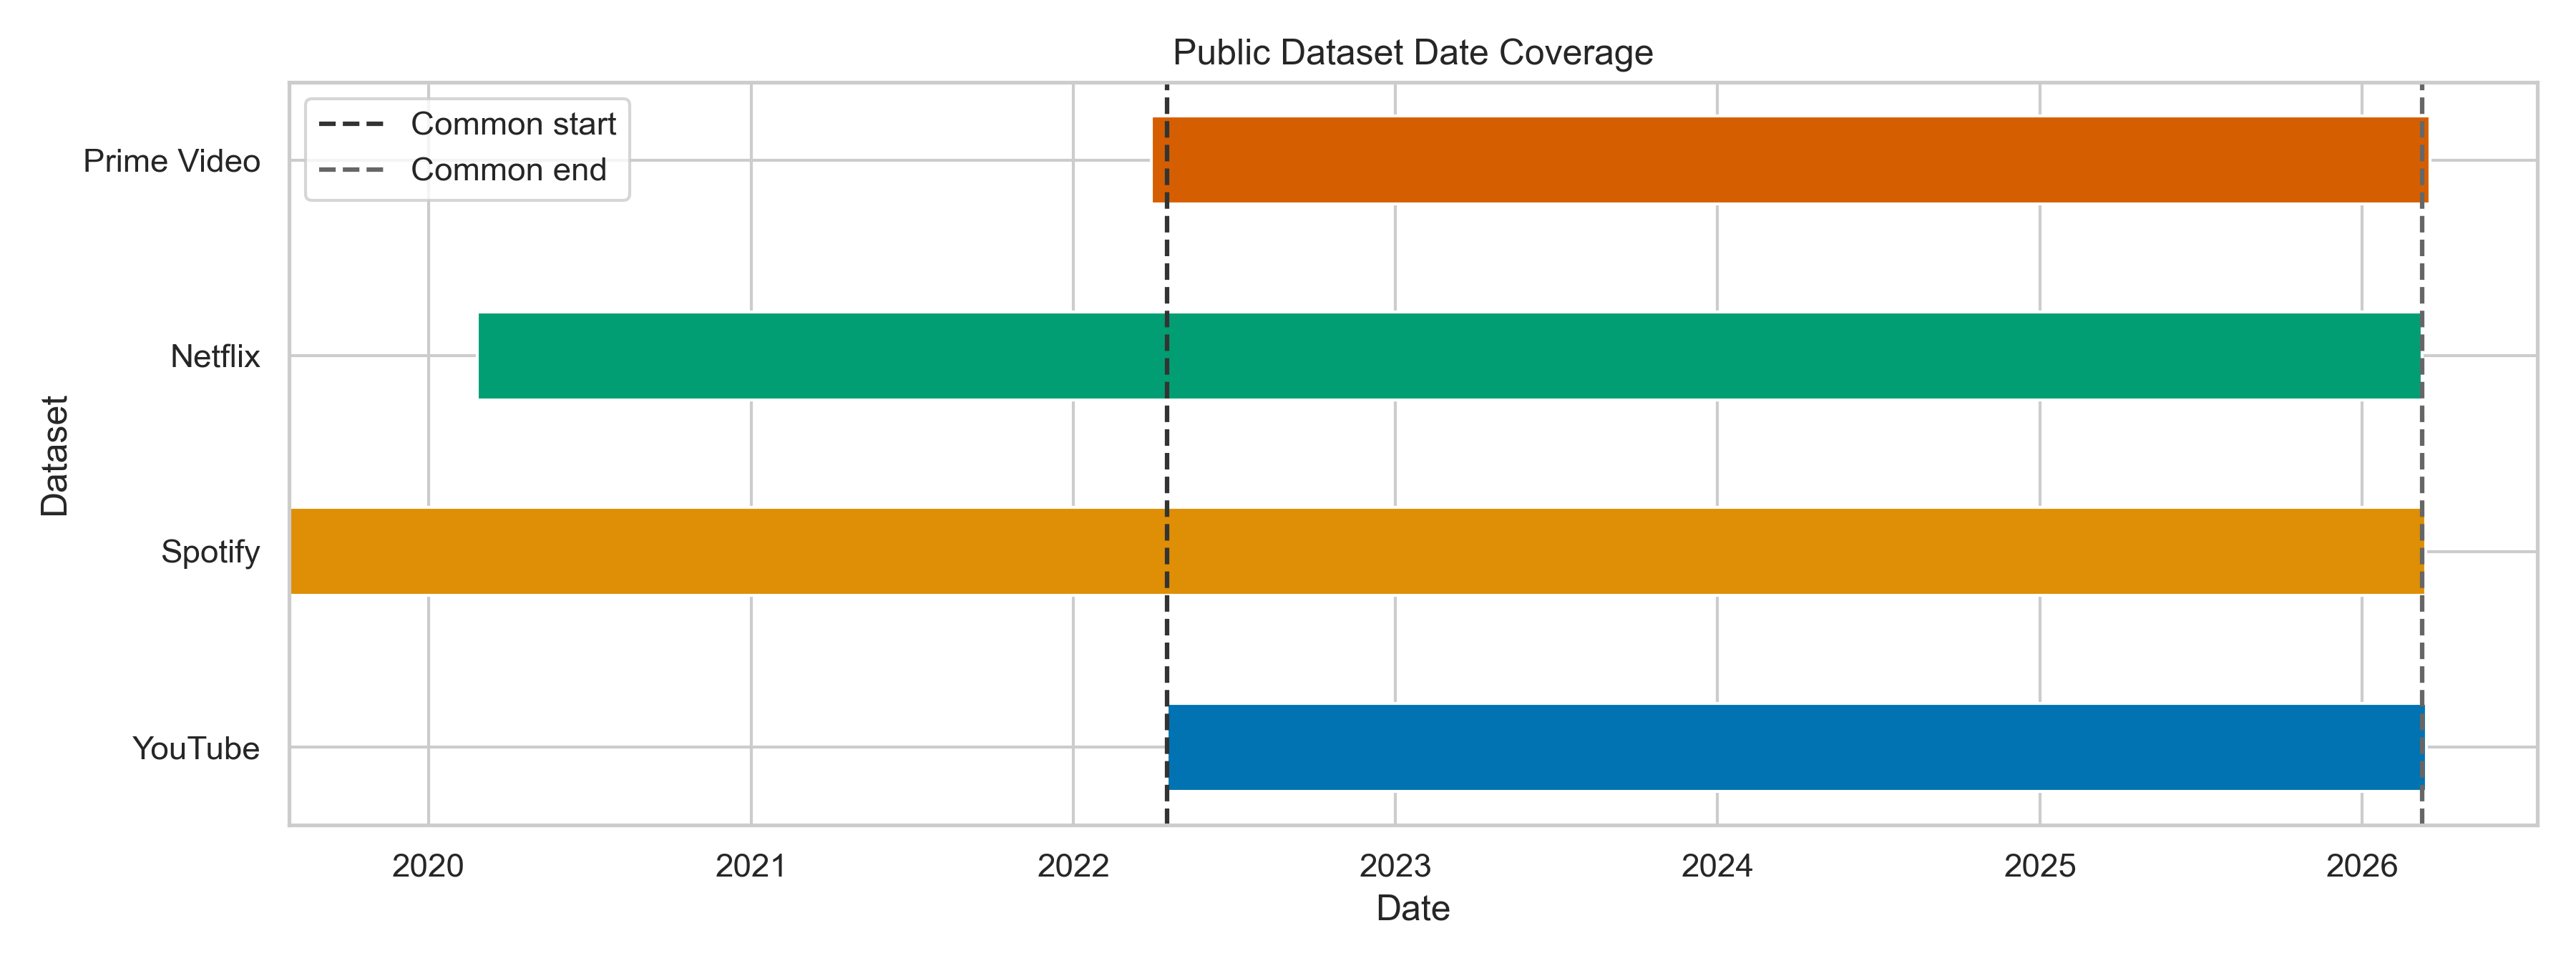
\includegraphics[width=0.88\textwidth]{../EDA/combined_images/combined_dataset_date_coverage.png}
\caption{Dataset date coverage. The common comparison window begins on 2022-04-17 and ends on 2026-03-10.}
\label{fig:coverage}
\end{figure}

\begin{figure}[H]
\centering
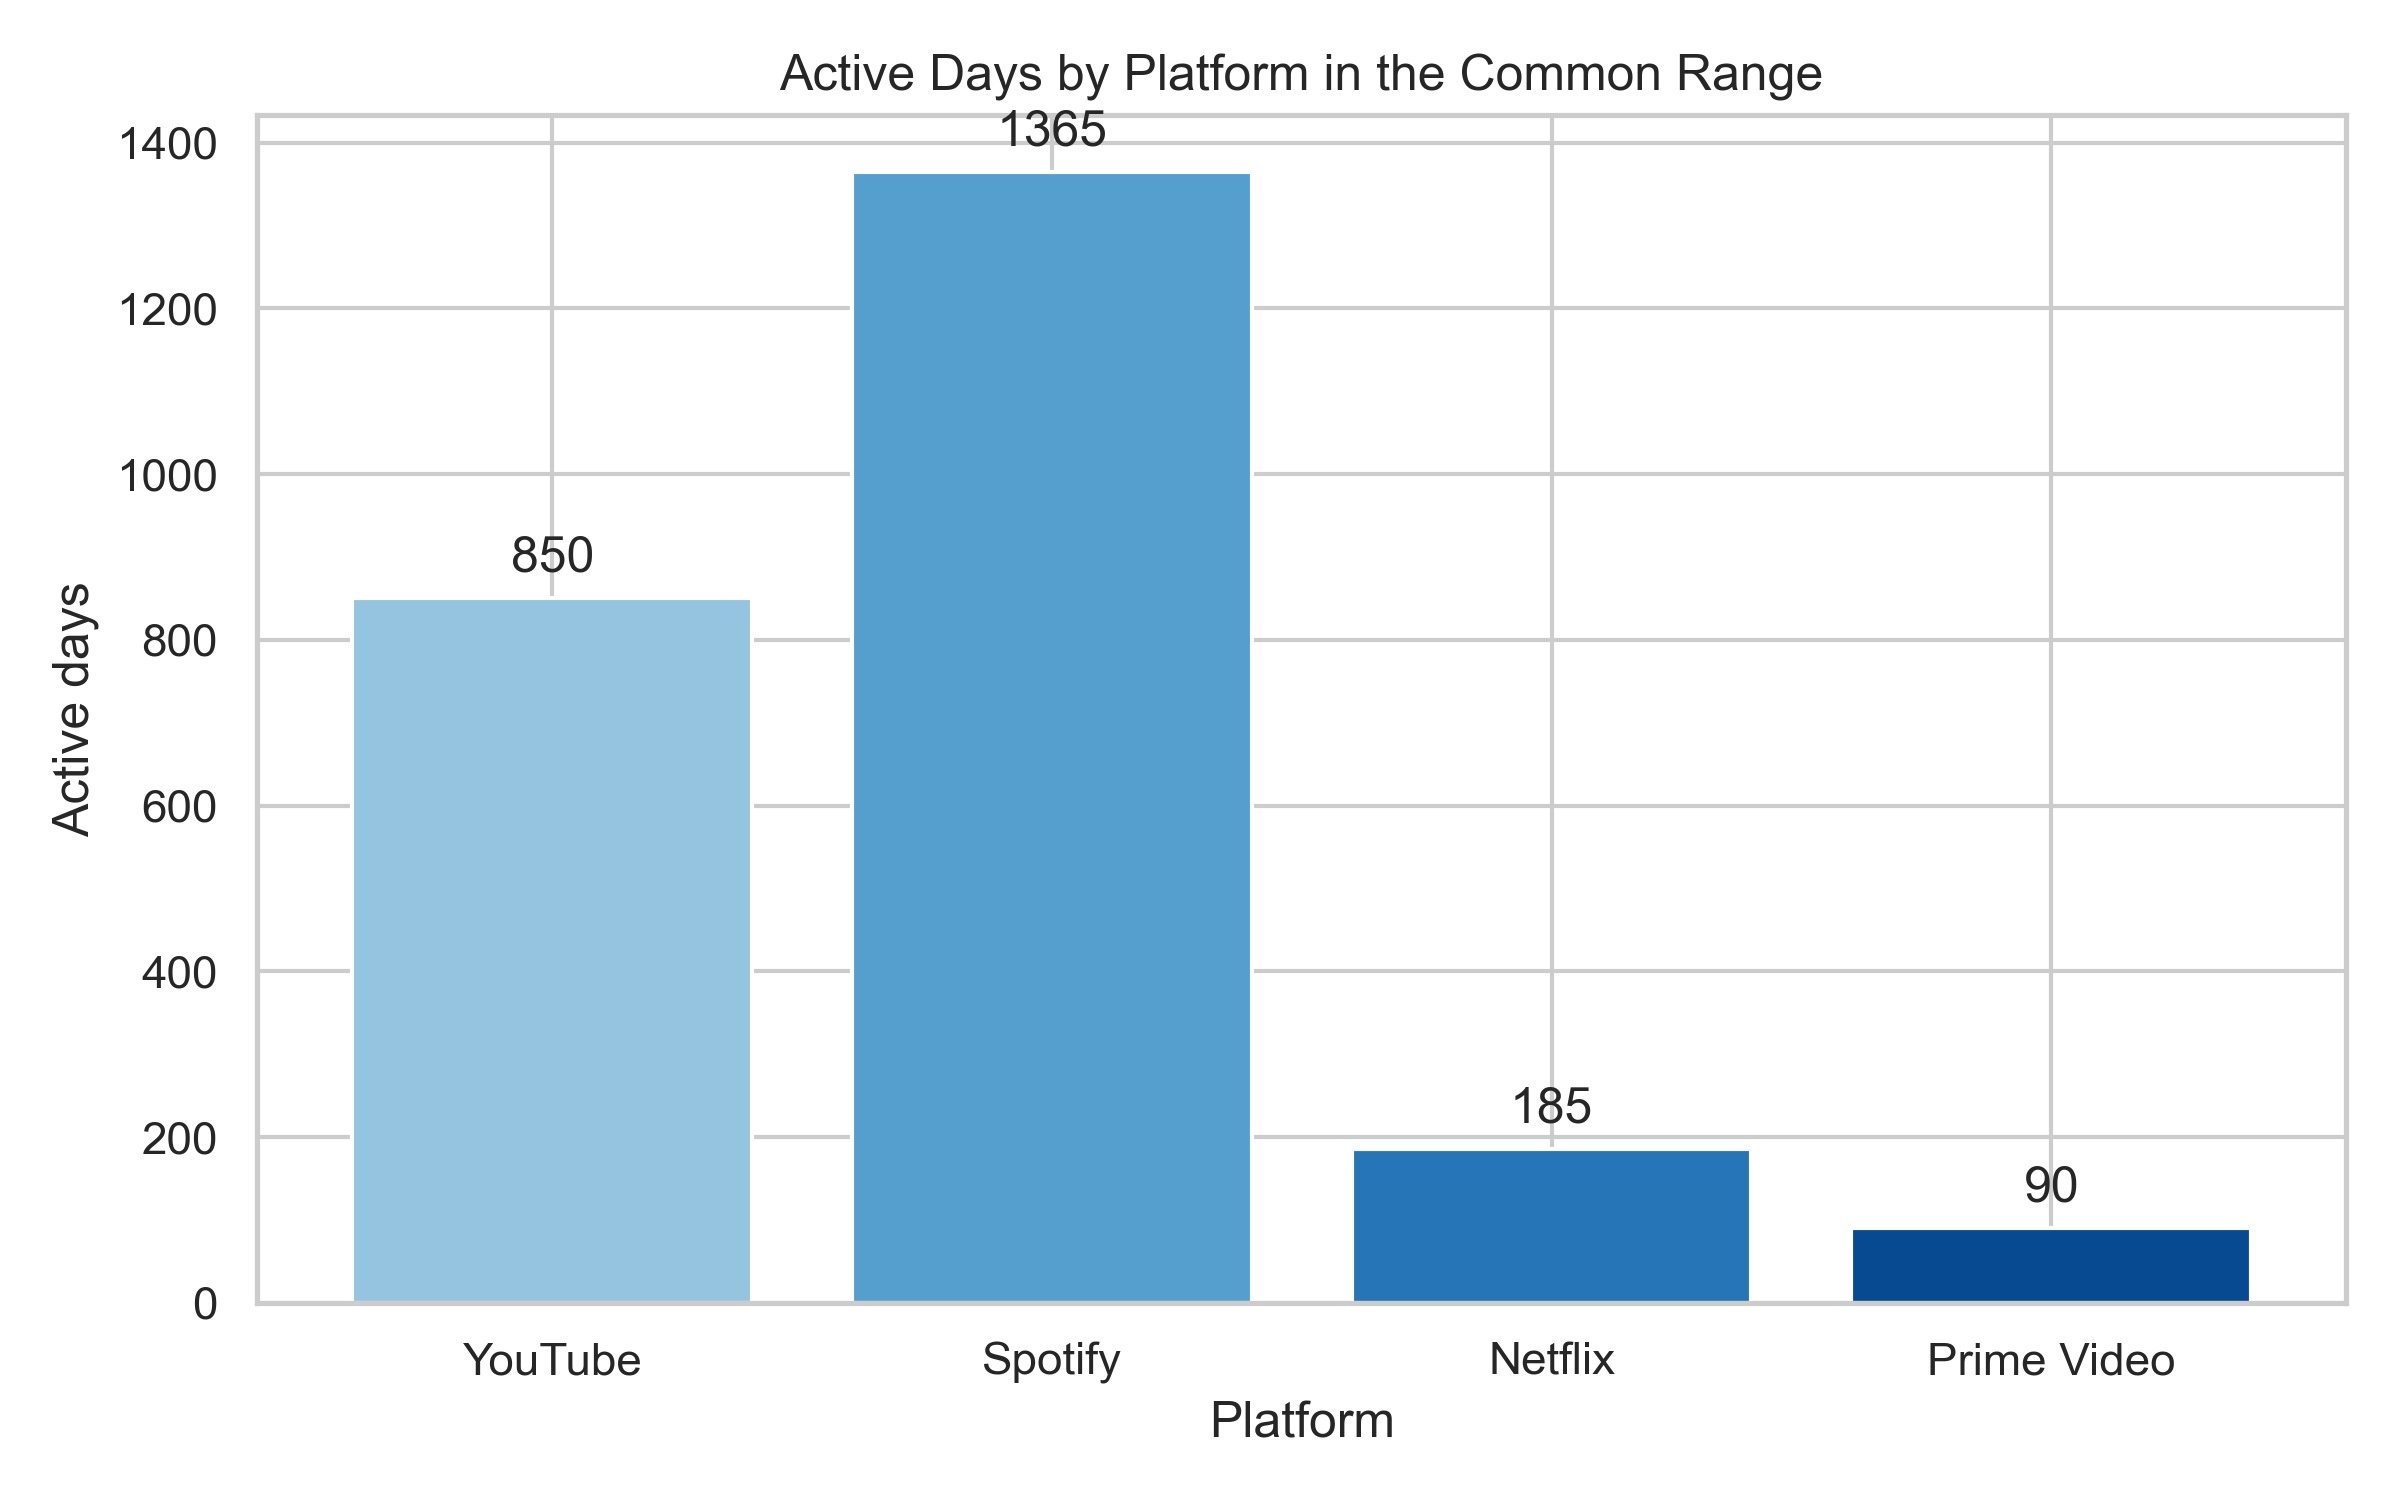
\includegraphics[width=0.88\textwidth]{../EDA/combined_images/combined_active_days_by_platform.png}
\caption{Active days by platform in the common date range. This highlights the difference between continuous platforms and sparse long-form viewing.}
\label{fig:active-days}
\end{figure}

\figref{fig:monthly-trends} shows that platform activity does not follow one shared pattern. YouTube, Spotify, and long-form streaming peak in different periods. \figref{fig:correlation} shows that variables within the same platform are more strongly related than variables across different platforms. \figref{fig:after2130} is especially important because it connects directly to the late-evening hypothesis.

\begin{figure}[H]
\centering
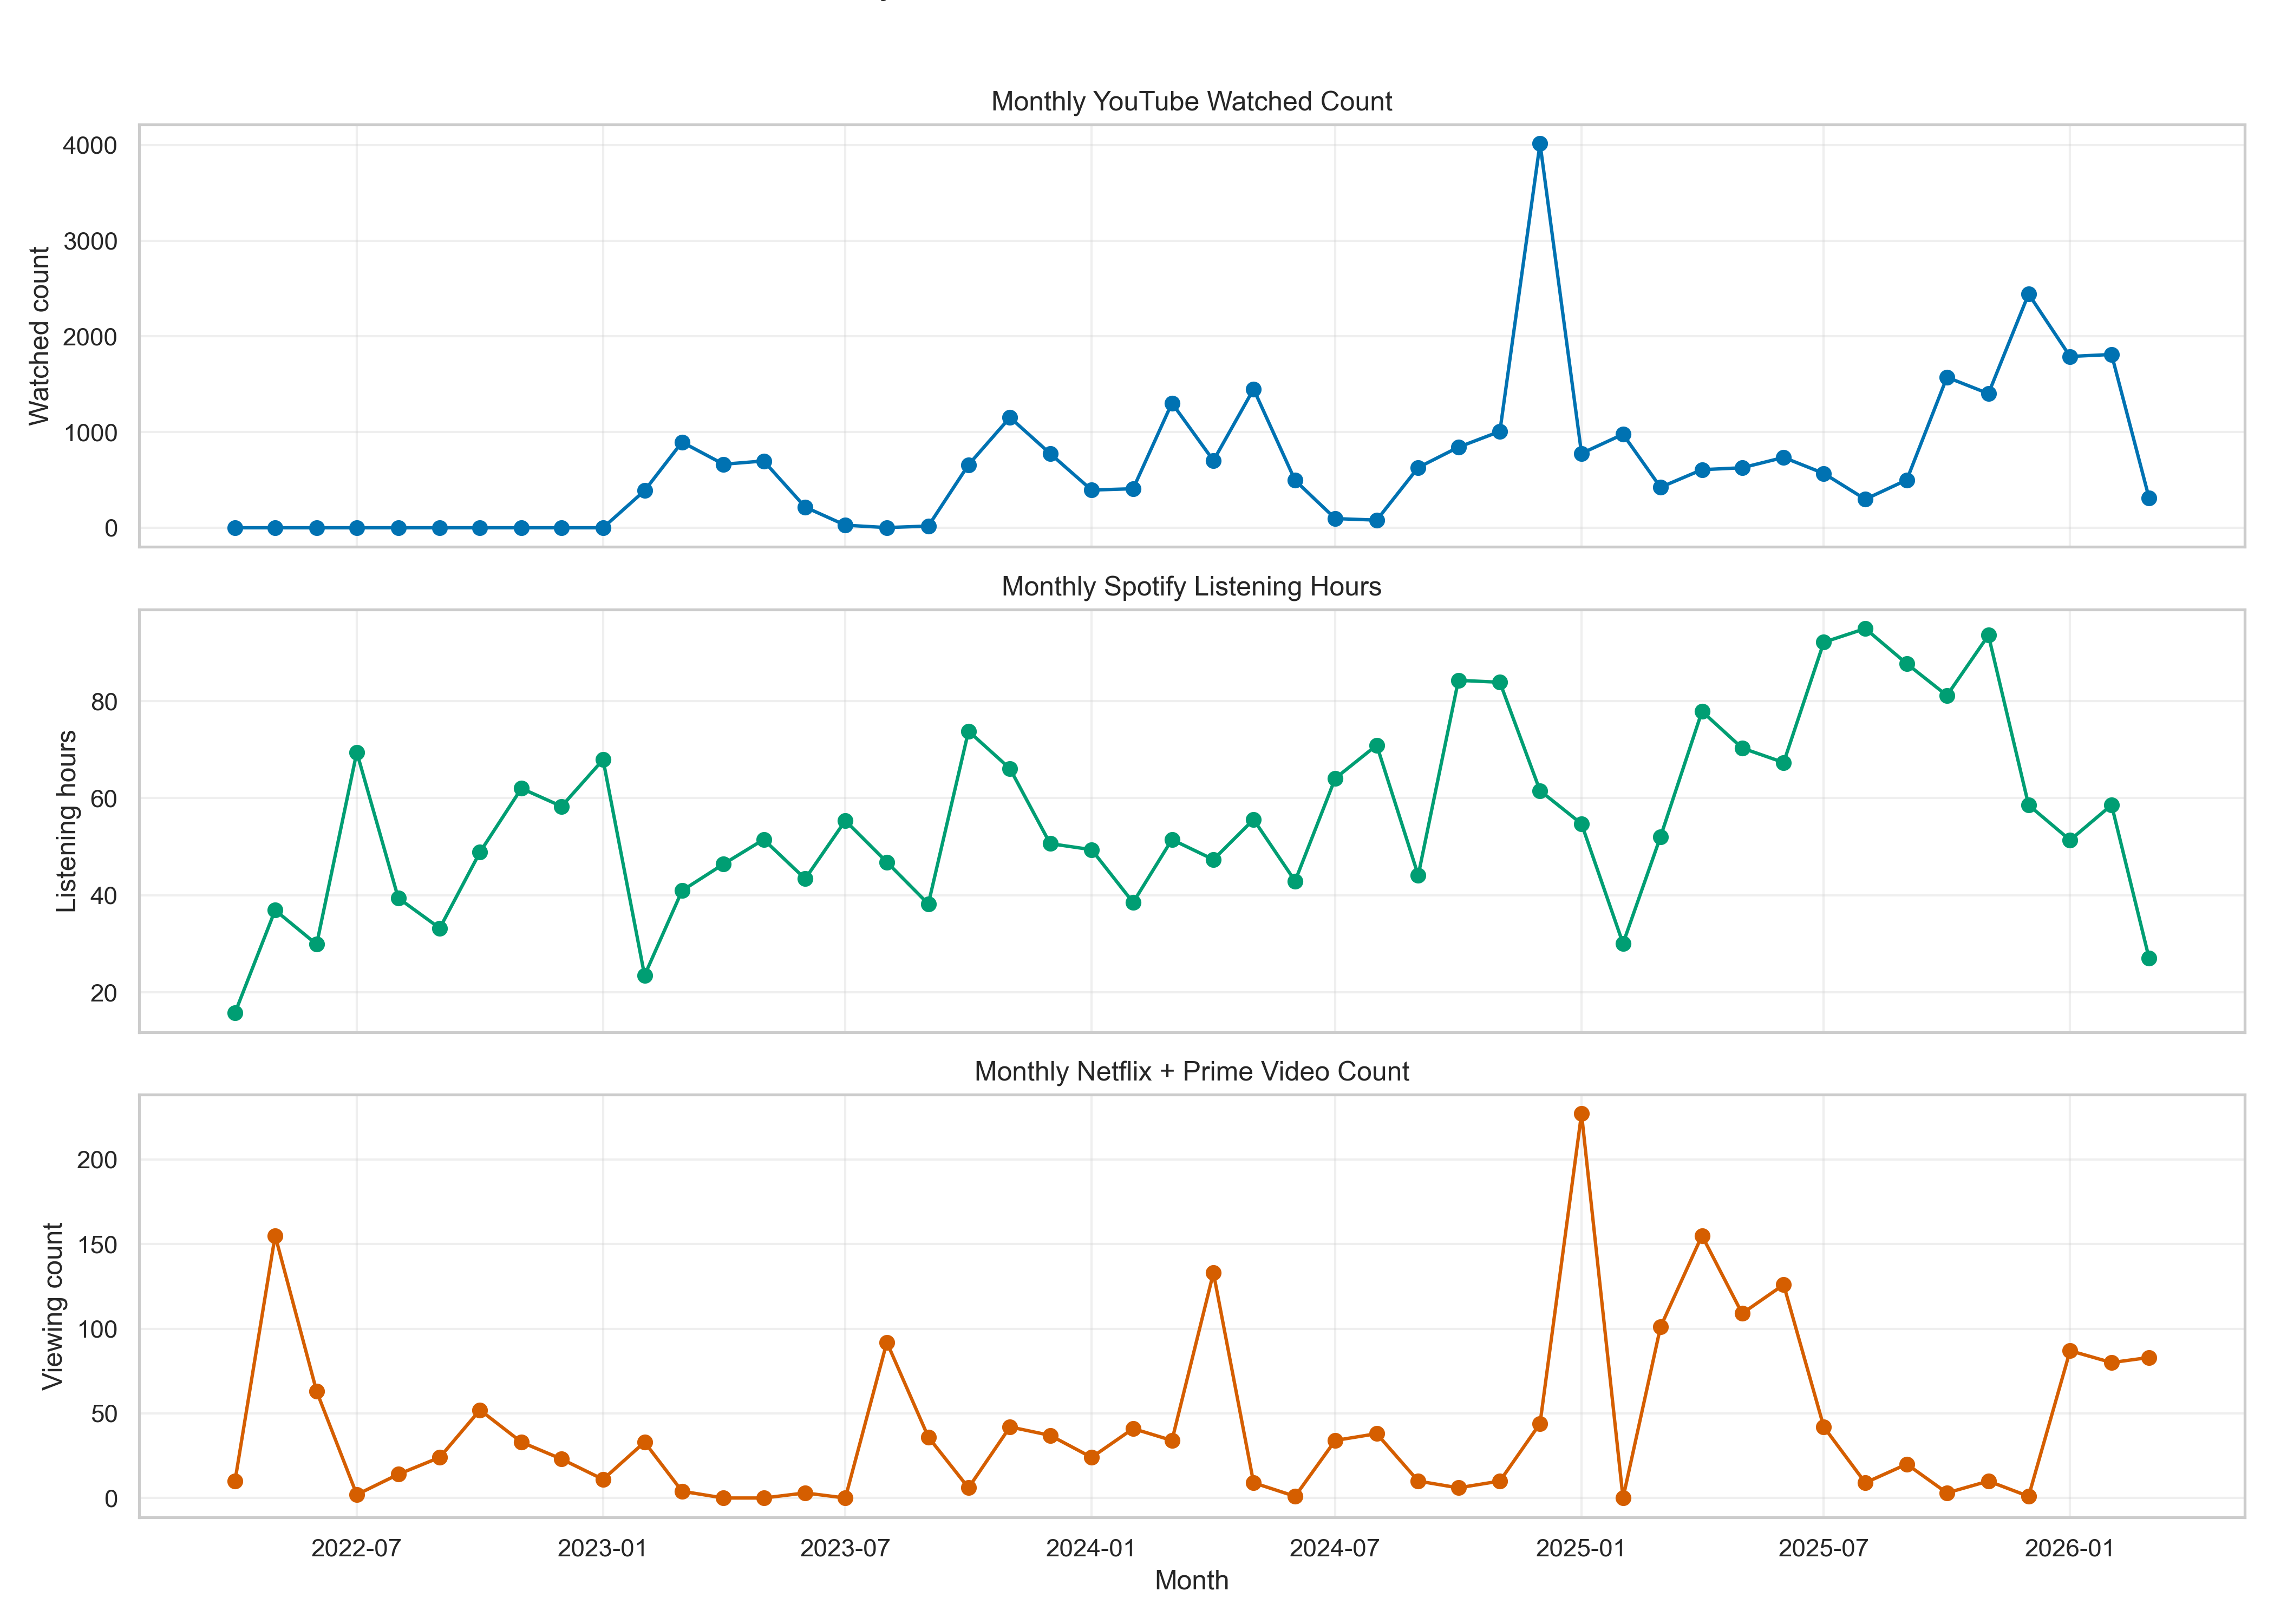
\includegraphics[width=0.88\textwidth]{../EDA/combined_images/combined_monthly_cross_platform_trends.png}
\caption{Monthly cross-platform trends. Separate panels are used because platform units differ.}
\label{fig:monthly-trends}
\end{figure}

\begin{figure}[H]
\centering
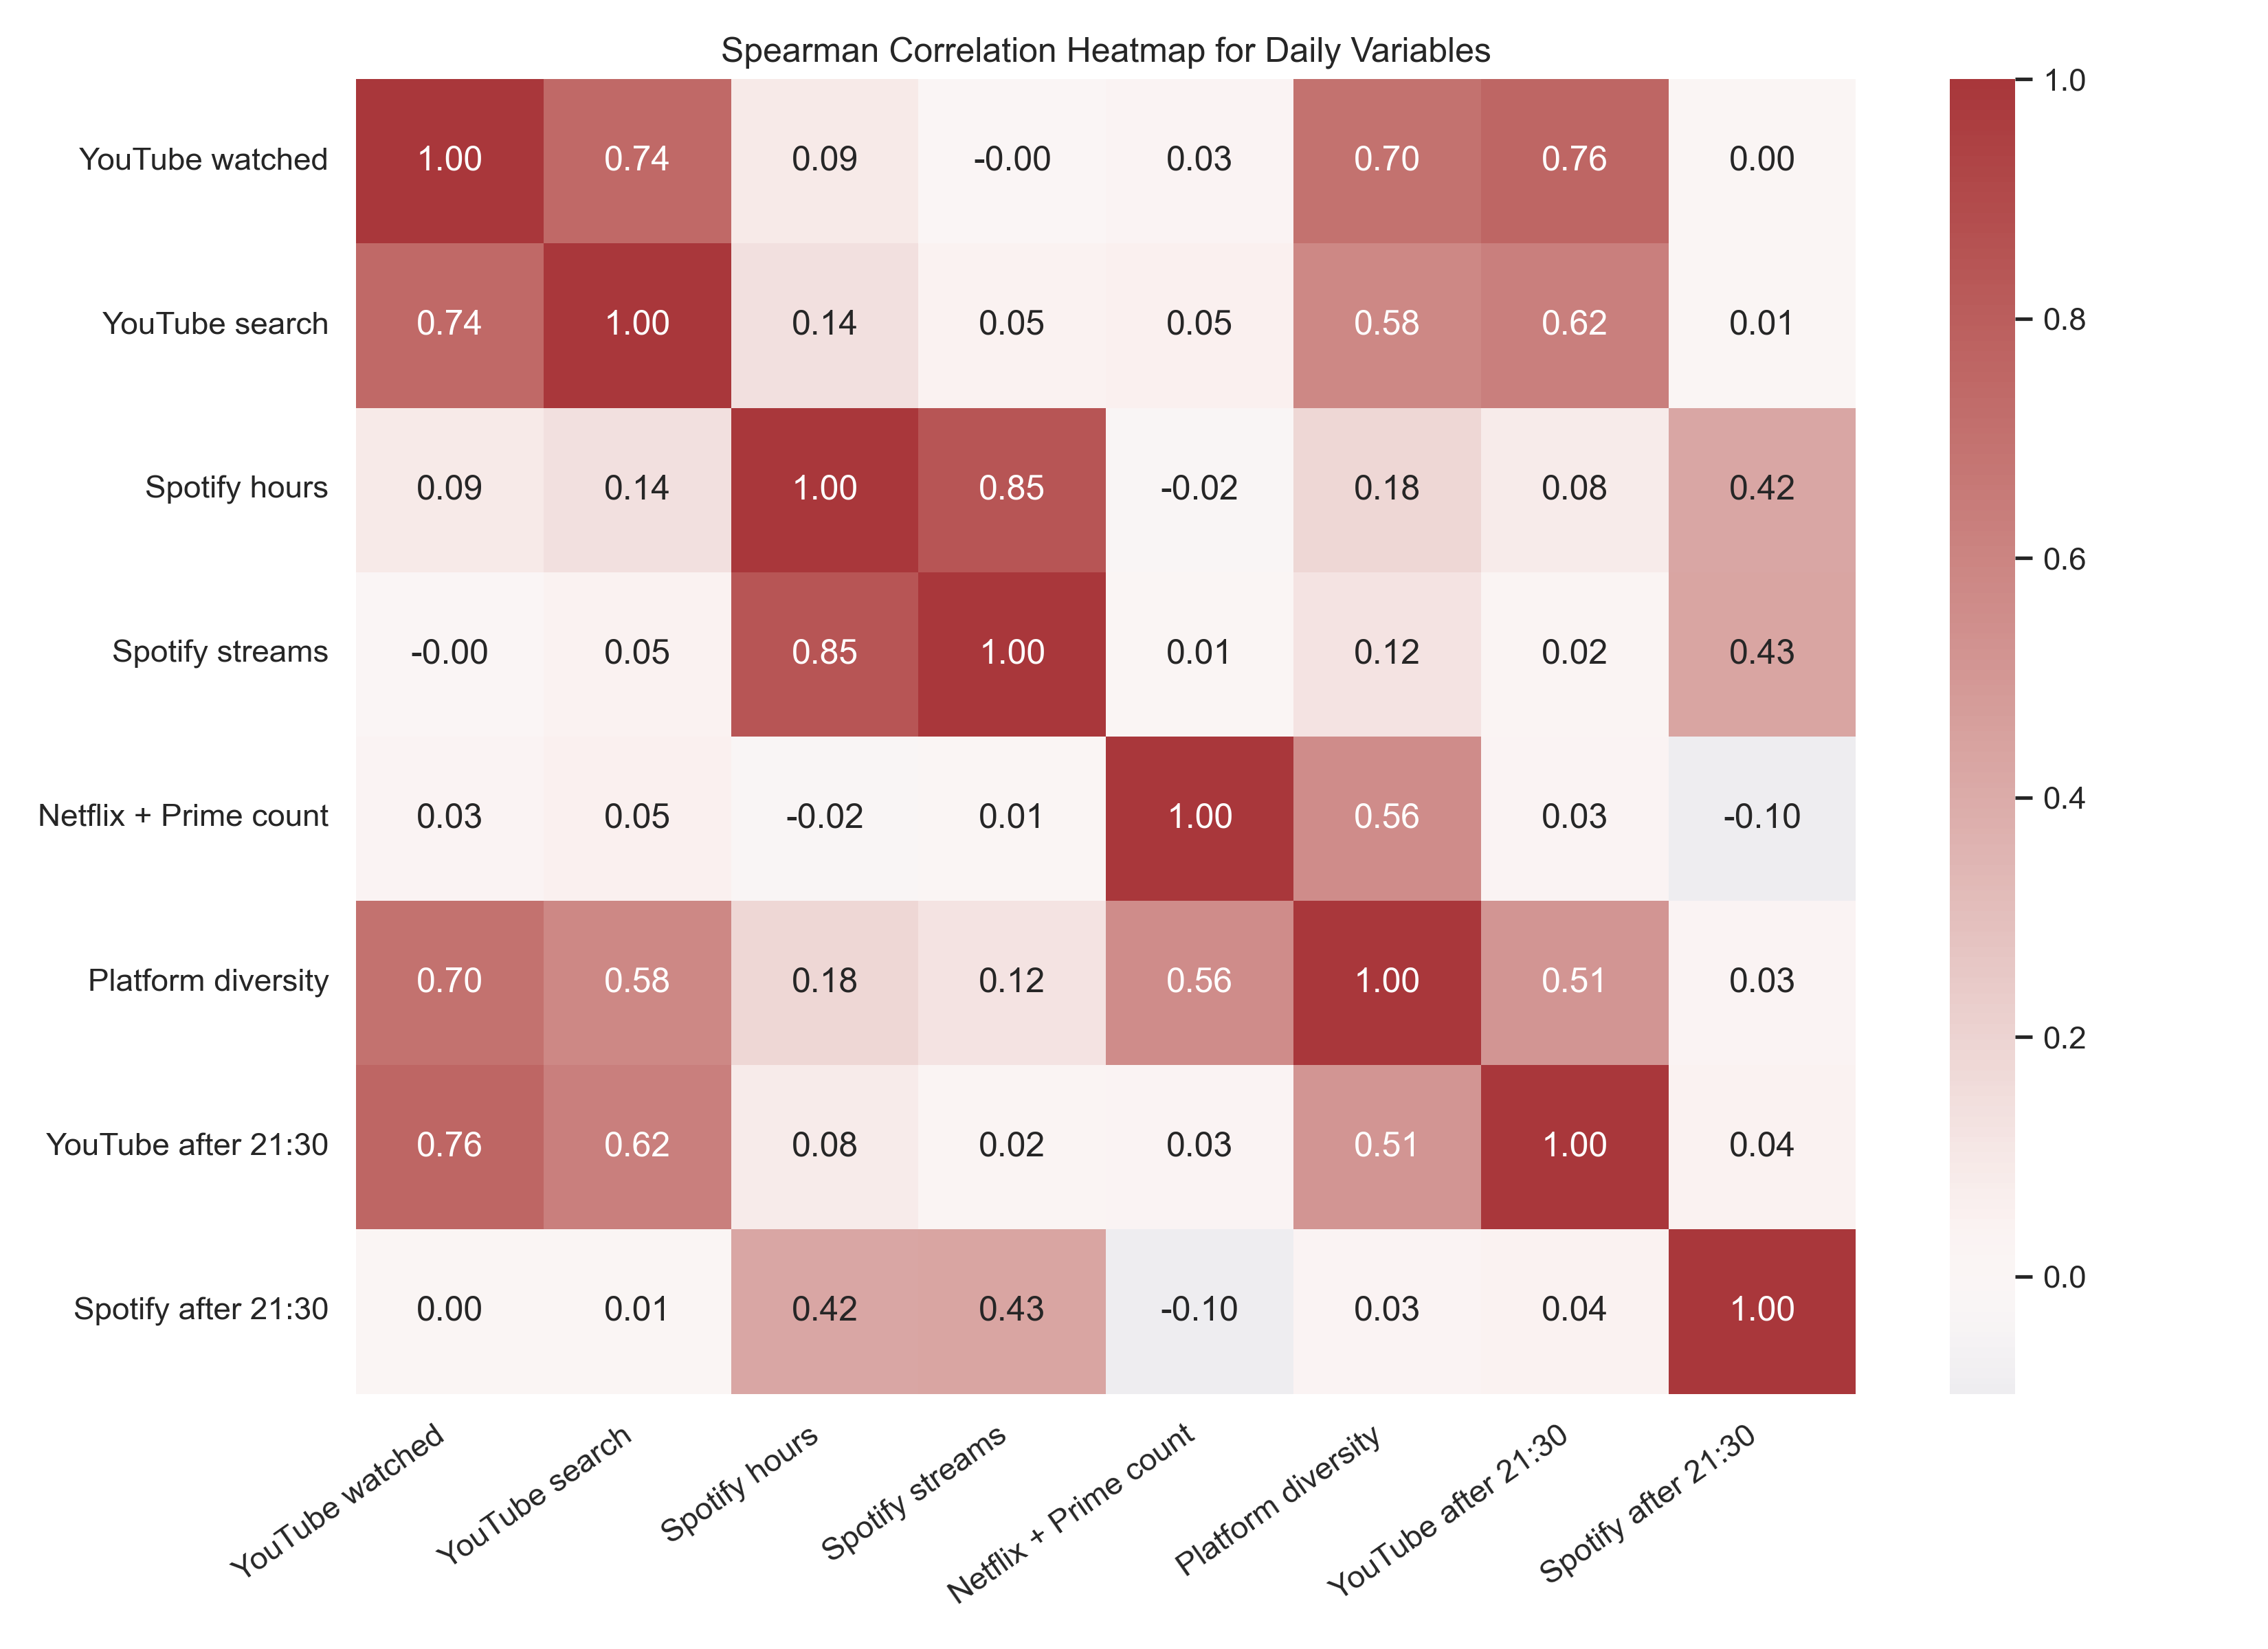
\includegraphics[width=0.88\textwidth]{../EDA/combined_images/combined_daily_variable_correlation_heatmap.png}
\caption{Daily-variable correlation heatmap. Same-platform variables move together more strongly than most cross-platform pairs.}
\label{fig:correlation}
\end{figure}

\begin{figure}[H]
\centering
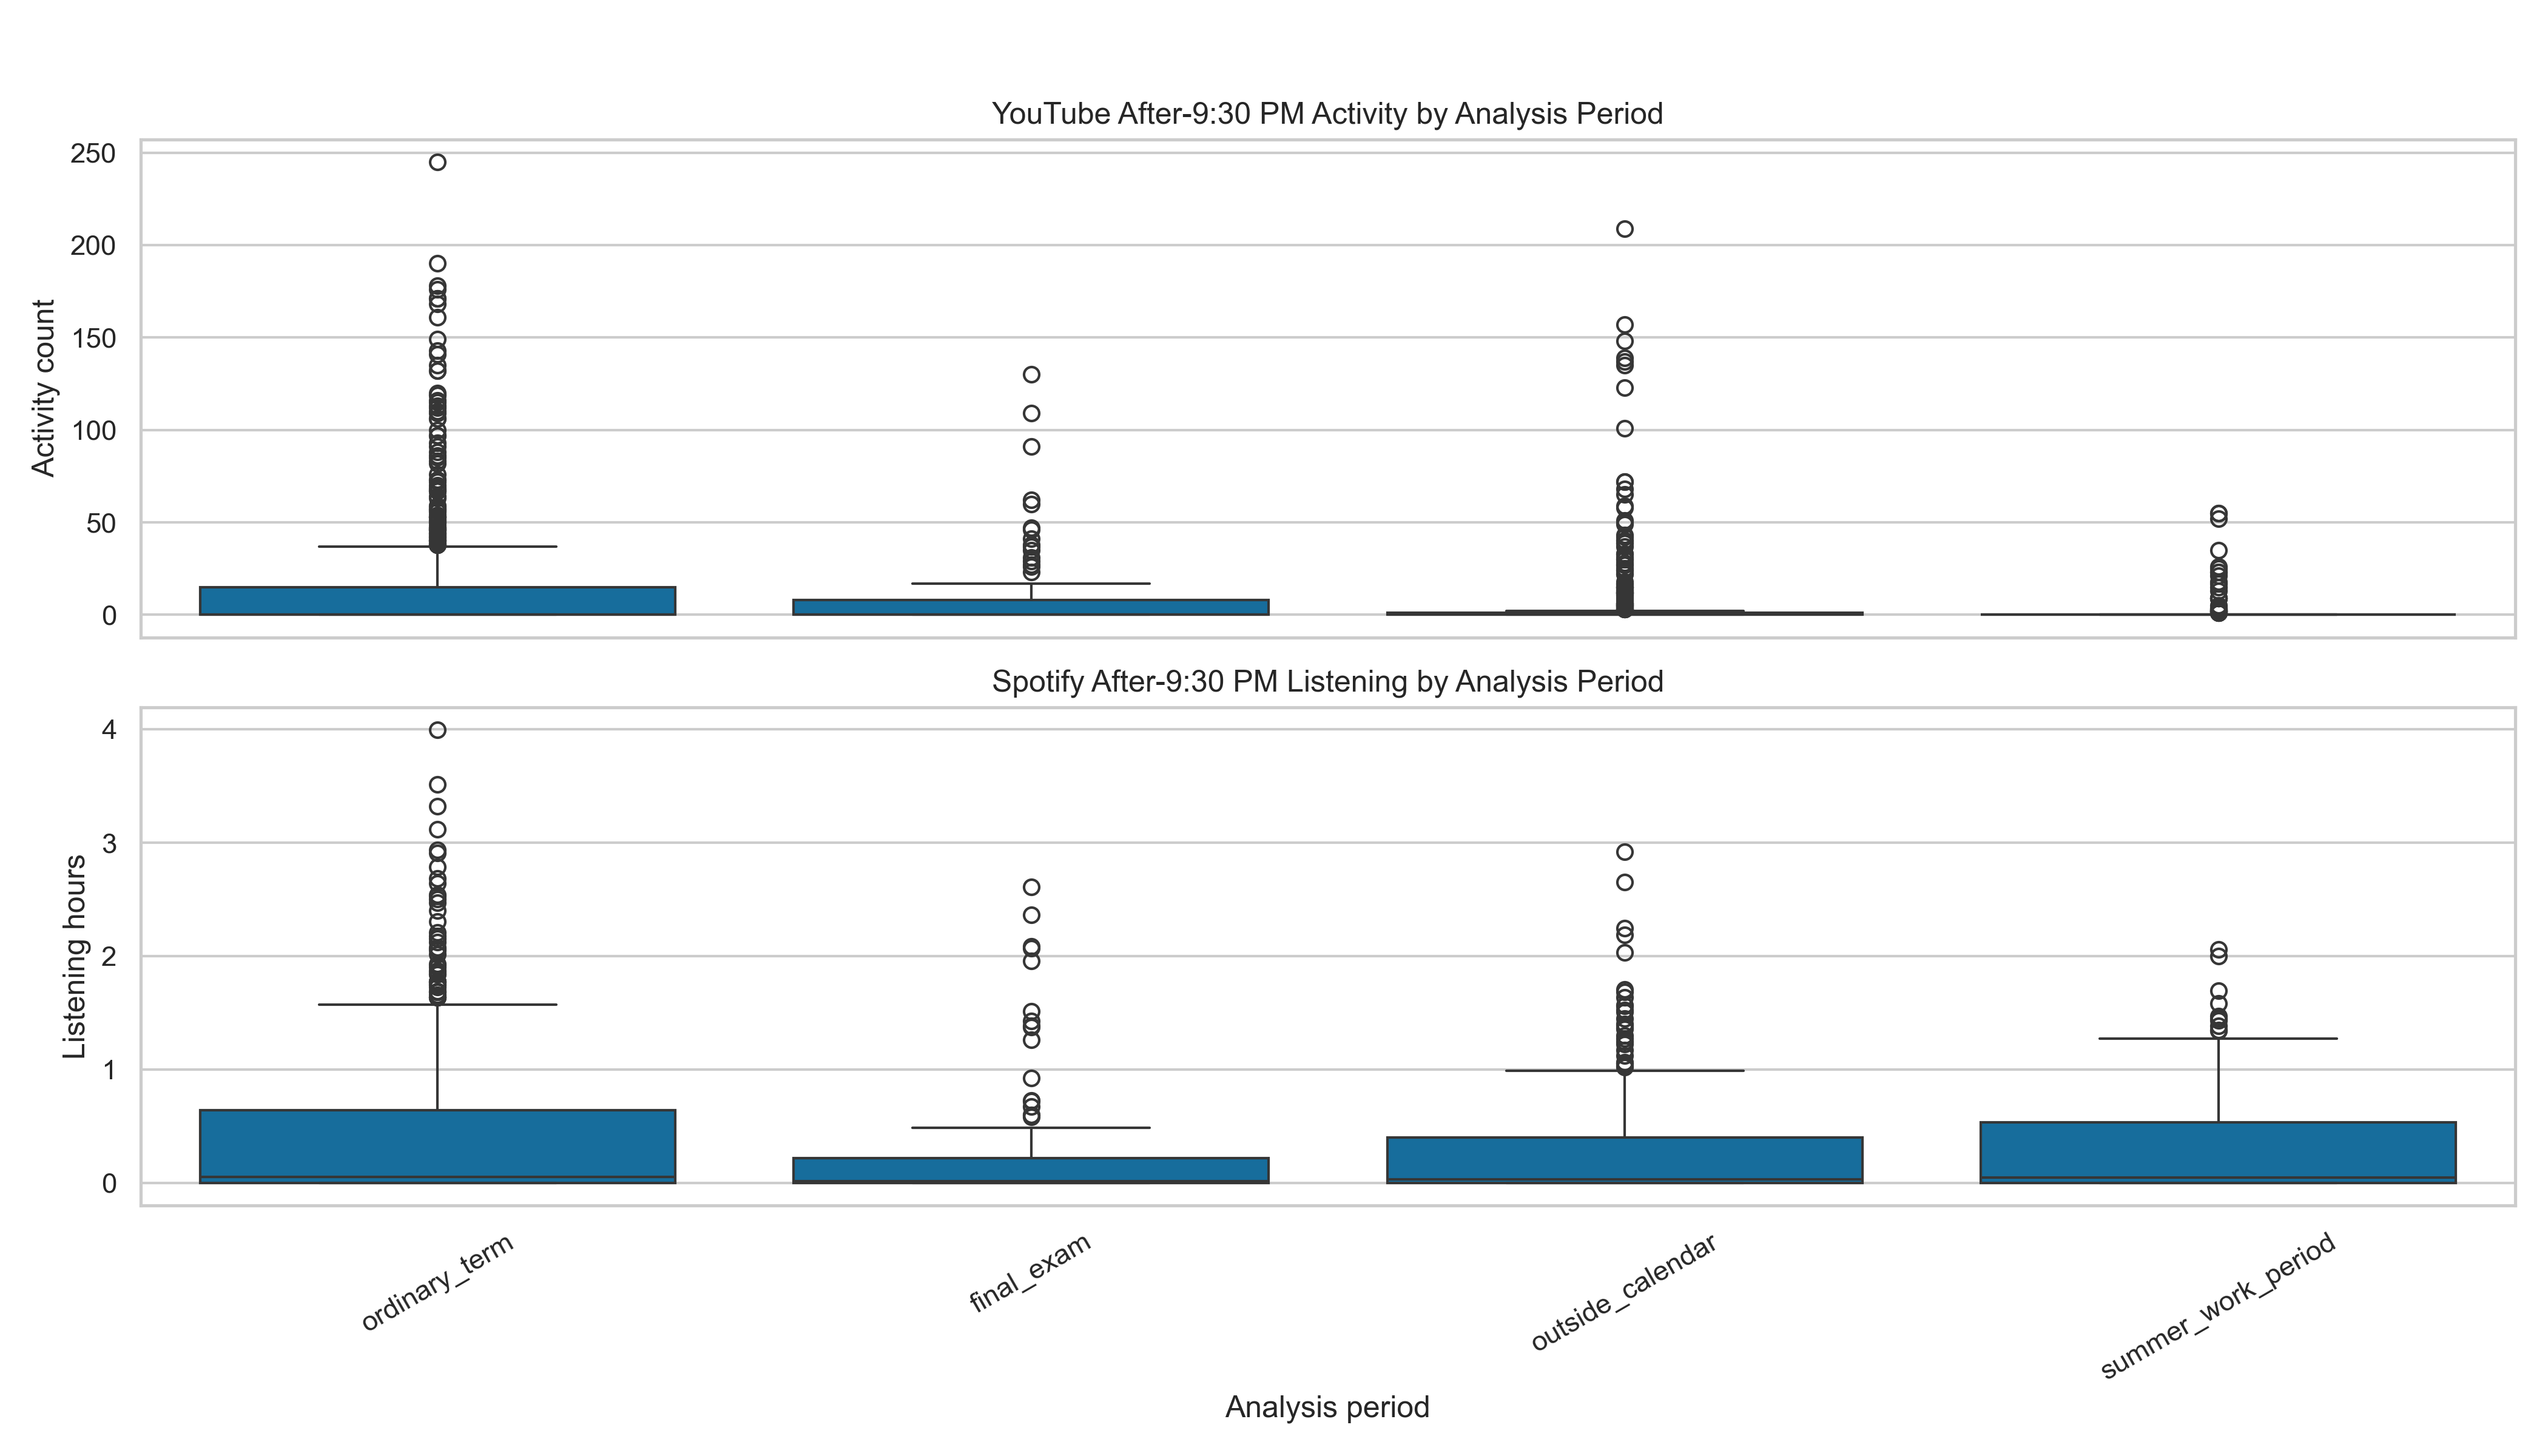
\includegraphics[width=0.88\textwidth]{../EDA/combined_images/combined_after_2130_by_analysis_period_boxplots.png}
\caption{After-21:30 activity by academic period. This figure supports the late-evening entertainment analysis.}
\label{fig:after2130}
\end{figure}

\subsection{Hypothesis Testing}

The formal tests use the combined daily panel. For final-exam comparisons, I compared only \texttt{final\_exam} and \texttt{ordinary\_term}. Outside-calendar and summer-work days were kept for descriptive context but excluded from the final-versus-ordinary hypothesis tests.

Because the daily activity variables are skewed and zero-heavy, I used one-sided Mann--Whitney U tests for group comparisons. For same-day Spotify and YouTube co-usage, I used one-sided Spearman correlation because it tests monotonic association without assuming a linear relationship.

\begin{table}[H]
\centering
\scriptsize
\caption{Hypothesis tests used in the project.}
\label{tab:hypotheses}
\begin{tabularx}{\textwidth}{p{0.15\textwidth} X X p{0.18\textwidth}}
\toprule
\textbf{Hypothesis} & \textbf{Null hypothesis (H0)} & \textbf{Alternative hypothesis (H1)} & \textbf{Method}\\
\midrule
H1: Entertainment usage during academic pressure & Platform activity does not differ between final-exam days and ordinary-term days. & Final-exam days have lower platform activity. & One-sided Mann--Whitney U, tested separately by platform.\\
H2: Platform diversity during academic pressure & Platform diversity does not differ between final-exam days and ordinary-term days. & Platform diversity is lower during finals. & One-sided Mann--Whitney U.\\
H3: Long-form streaming and YouTube activity & YouTube watched count does not differ between Netflix + Prime active and inactive days. & YouTube watched count is lower on Netflix + Prime active days. & One-sided Mann--Whitney U.\\
H4: Spotify and YouTube co-usage & Spotify hours are not associated with YouTube watched count. & Spotify hours have a positive association with YouTube watched count. & One-sided Spearman correlation.\\
H5: After-9:30 PM entertainment during finals & Late-evening entertainment share does not differ between final-exam days and ordinary-term days. & Late-evening share is lower during finals. & One-sided Mann--Whitney U, tested separately for YouTube and Spotify.\\
\bottomrule
\end{tabularx}
\end{table}

\begin{table}[H]
\centering
\scriptsize
\caption{Current hypothesis test results.}
\label{tab:hypothesis-results}
\begin{tabularx}{\textwidth}{p{0.07\textwidth} p{0.27\textwidth} p{0.17\textwidth} r X}
\toprule
\textbf{Hyp.} & \textbf{Outcome} & \textbf{Decision} & \textbf{Raw p-value} & \textbf{Interpretation}\\
\midrule
H1 & YouTube watched count & Do not reject H0 & 0.0908 & Lower during finals on average, but not enough evidence to reject H0.\\
H1 & Spotify listening hours & Do not reject H0 & 0.0697 & Lower during finals on average, but not enough evidence to reject H0.\\
H1 & Netflix viewing count & Do not reject H0 & 0.8512 & Does not support the expected lower-finals direction.\\
H1 & Prime Video viewing count & Do not reject H0 & 0.3890 & Does not provide enough evidence for lower finals usage.\\
H2 & Distinct active entertainment platforms & Do not reject H0 & 0.1305 & Platform diversity did not significantly decrease during finals.\\
H3 & YouTube watched count on long-form active days & Do not reject H0 & 0.8731 & The direction was opposite to H1: mean YouTube watched count was higher on Netflix + Prime active days, so the lower-YouTube alternative could not be rejected.\\
H4 & Spotify hours and YouTube watched count & Reject H0 & 0.0002 & Statistically detectable but practically very weak positive association ($\rho=0.0934$).\\
H5 & YouTube after-21:30 activity share & Reject H0 & 0.0059 & YouTube late-evening share was lower during finals.\\
H5 & Spotify after-21:30 listening-hour share & Reject H0 & 0.0342 & Spotify late-evening listening share was lower during finals.\\
\bottomrule
\end{tabularx}
\end{table}

\begin{figure}[H]
\centering
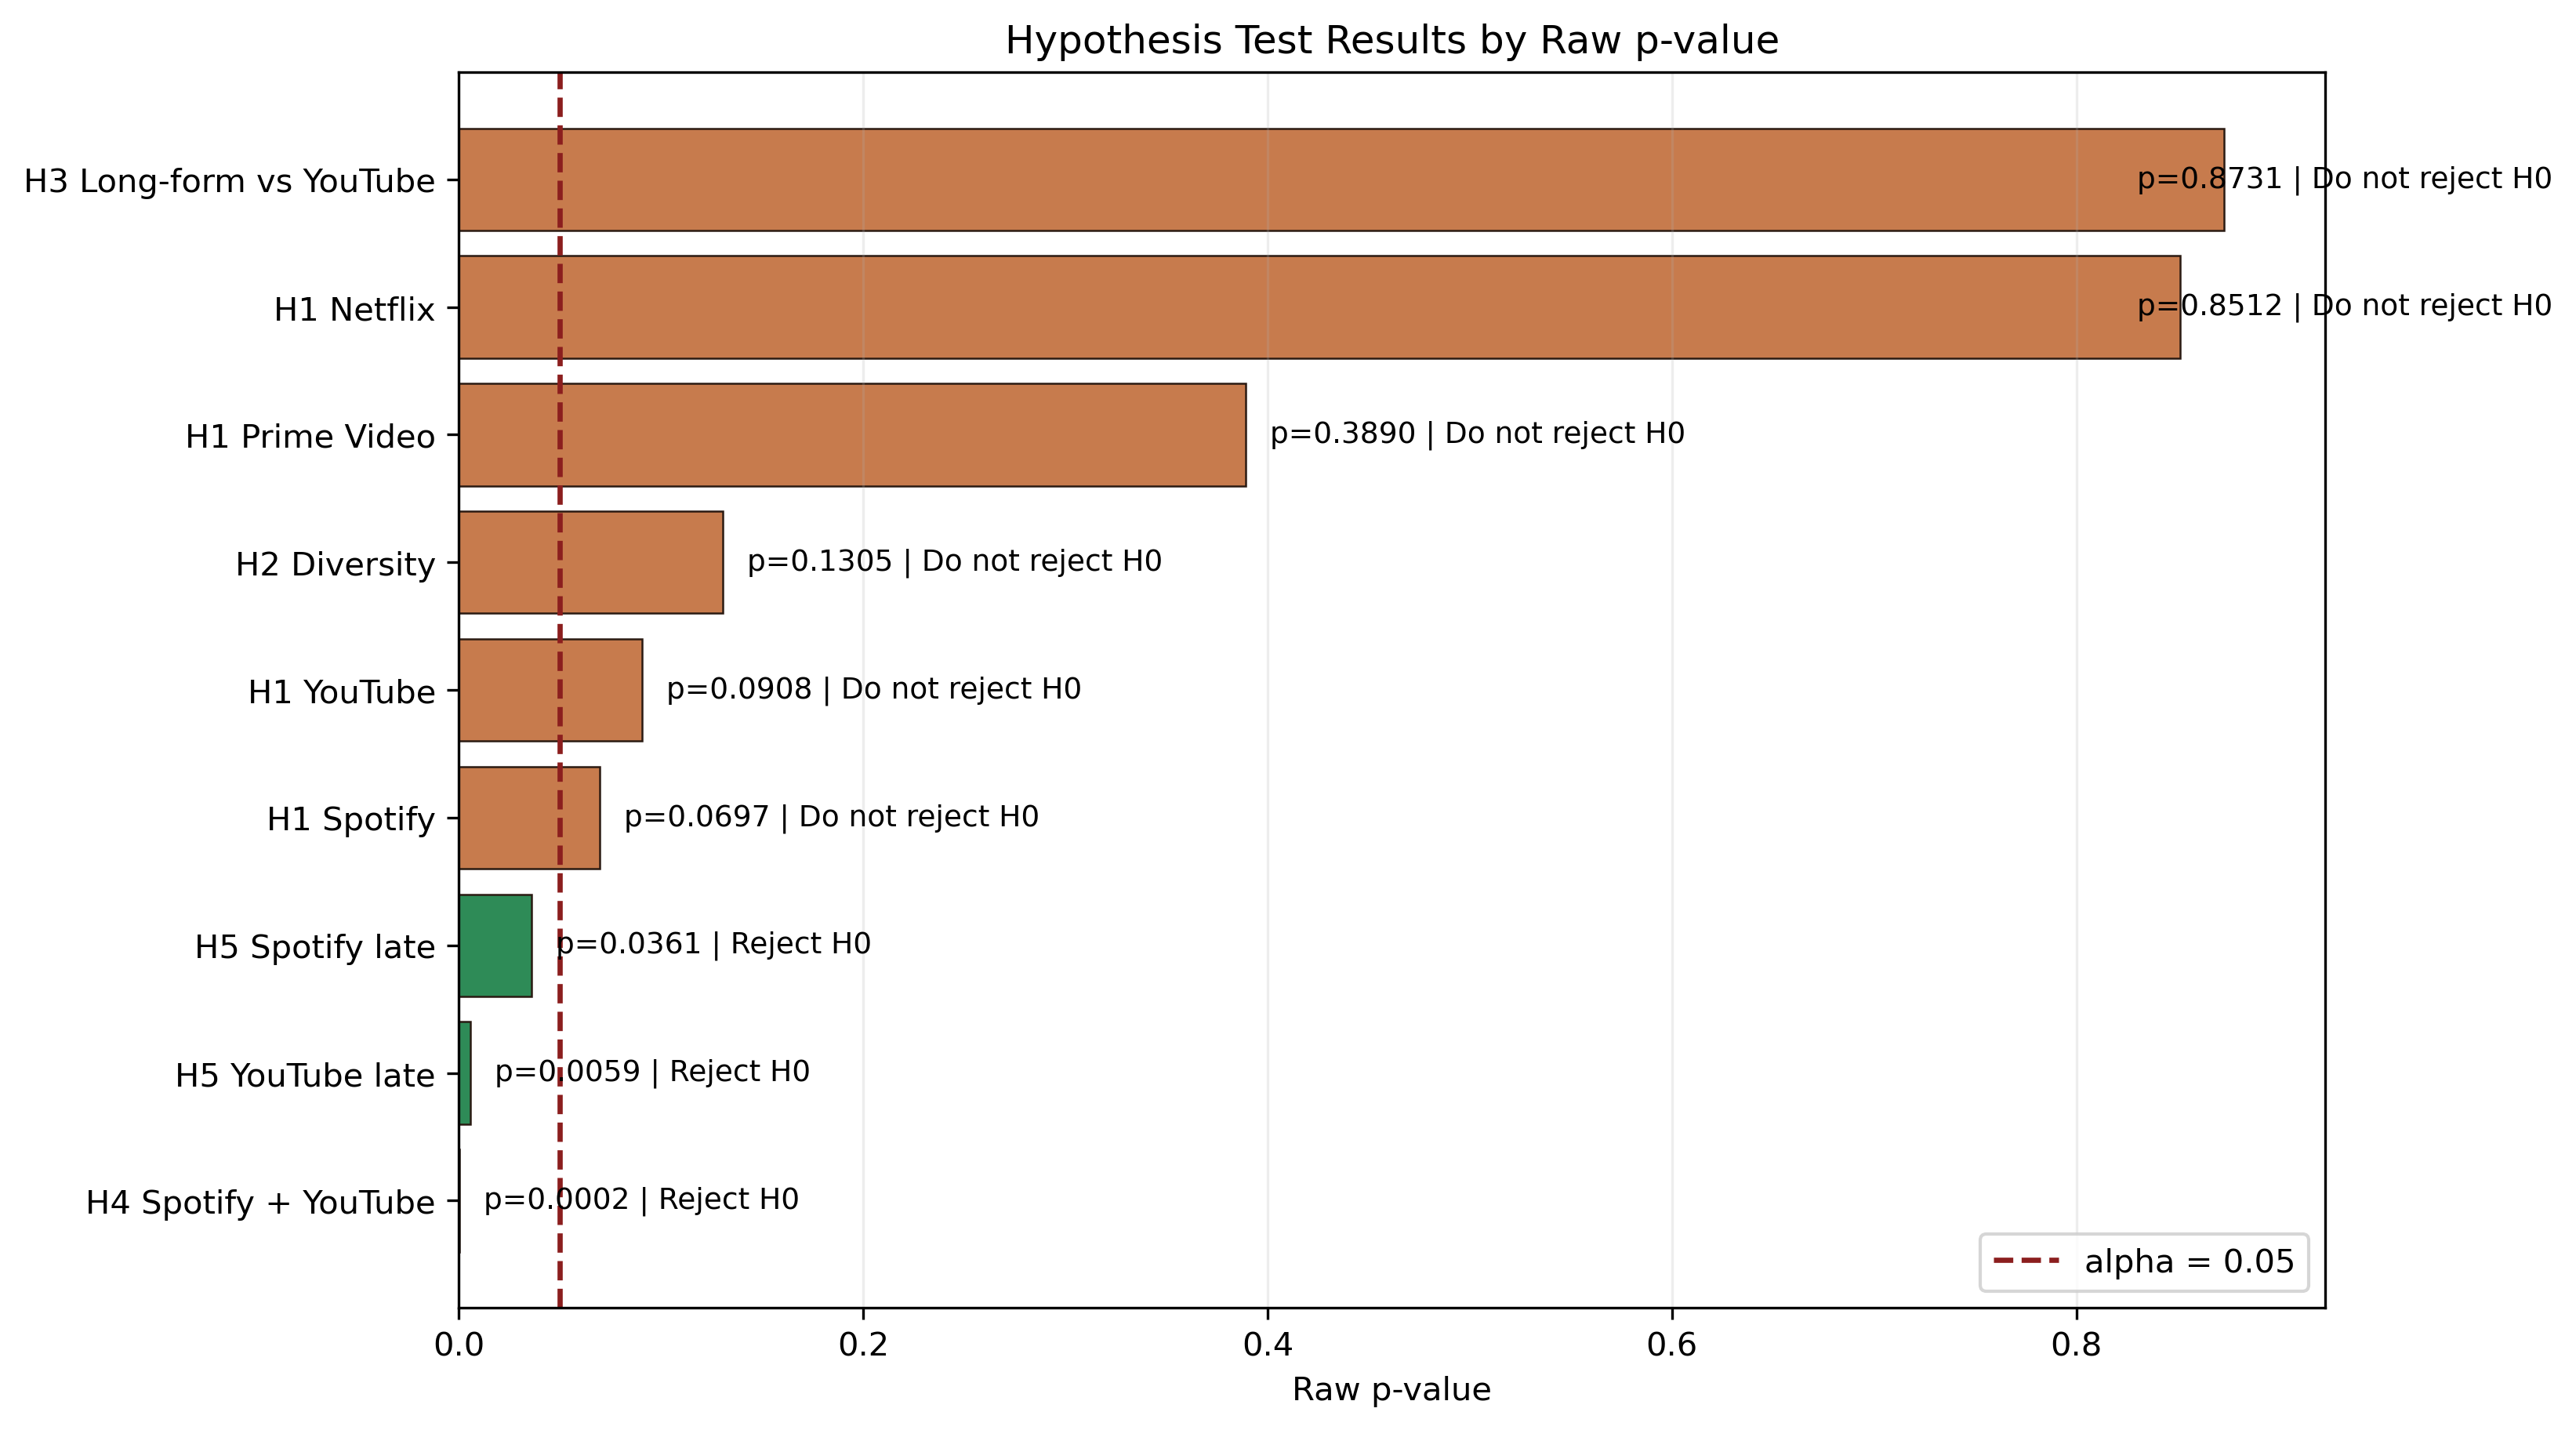
\includegraphics[width=0.9\textwidth]{../Hypothesis_Testing/hypothesis_results_decision_plot.png}
\caption{Hypothesis test results by raw p-value. The dashed line marks $\alpha=0.05$.}
\label{fig:hypothesis-plot}
\end{figure}

The broad entertainment-usage hypothesis was not supported strongly enough when tested platform by platform. H3 also moved opposite to the stated alternative: YouTube watched count was higher on Netflix + Prime active days on average, so the test could not support the lower-YouTube direction. However, late-evening activity was significantly lower during finals for both YouTube and Spotify. The Spotify--YouTube co-usage test was also significant, but the Spearman correlation was only $\rho=0.0934$, which is practically very weak and likely detectable mainly because the daily panel has 1,424 observations.

\subsection{Machine Learning}

The machine learning notebook is \texttt{MachineLearning/machinelearning.ipynb}, and the newest output folder is \texttt{MachineLearning/results2/}. The goal was to test whether daily entertainment variables can classify academic periods.

The classification tasks were separated into three parts: final exam versus ordinary term, summer work versus ordinary term, and all-period classification. The supervised models use an 80/20 stratified train/test split. Hyperparameter tuning is performed with GridSearchCV and 5-fold StratifiedKFold on the training set only; the test set is kept separate for final evaluation. Macro F1-score is the main selection metric because the classes are imbalanced. Because nearby days are autocorrelated, the random split likely makes these scores optimistic relative to a chronological held-out split.

\begin{table}[H]
\centering
\footnotesize
\caption{Machine learning classification tasks.}
\label{tab:ml-tasks}
\begin{tabularx}{\textwidth}{>{\raggedright\arraybackslash}X >{\raggedright\arraybackslash}X >{\raggedright\arraybackslash}X r r r}
\toprule
\textbf{Task} & \textbf{Classes} & \textbf{Full Class Balance} & \textbf{Full} & \textbf{Train} & \textbf{Test}\\
\midrule
Final Exam vs Ordinary Term & \texttt{ordinary\_term}, \texttt{final\_exam} & 775 ordinary, 97 final (11.1\% final) & 872 & 697 & 175\\
Summer Work vs Ordinary Term & \texttt{ordinary\_term}, \texttt{summer\_work\_period} & 775 ordinary, 204 summer (20.8\% summer) & 979 & 783 & 196\\
All Periods Classification & \texttt{ordinary\_term}, \texttt{final\_exam}, \texttt{summer\_work\_period} & 775 ordinary, 97 final, 204 summer & 1,076 & 860 & 216\\
\bottomrule
\end{tabularx}
\end{table}

The final-exam task is especially imbalanced. In the held-out test set, there are 156 ordinary-term days and only 19 final-exam days. This explains why accuracy and macro F1 can move in opposite directions: the dummy classifier reaches 89.14\% accuracy by predicting the majority class, but its macro F1 is only 47.13\%. XGBoost and the ensemble reduce accuracy to 84.00\% while increasing macro F1 to 51.85\%, because they trade some majority-class correctness for a small amount of final-exam recall. XGBoost and the ensemble also produce identical final-task metrics to every reported decimal, which means the ensemble effectively inherited the same final test predictions as XGBoost.

The feature sets are not identical across all three tasks. The final-exam and all-period classifications use 11 daily activity features: YouTube watched/search counts, YouTube after-21:30 count, Spotify hours, Spotify stream count, Spotify unique tracks, Spotify after-21:30 hours, Netflix count, Prime Video count, Netflix plus Prime count, and daily distinct platform count. The summer-work classification uses those same 11 features plus two late-evening share features: \texttt{youtube\_after\_2130\_share} and \texttt{spotify\_after\_2130\_hour\_share}.

Because of this, the three ML tasks should not be read as a perfectly identical feature-set comparison. The summer-work task is still useful, but its stronger result may partly come from having the two additional share features. If the feature set were reduced to the same 11 columns for every task, the summer-work score could change. Therefore, I interpret the summer result as evidence that the task-specific feature set captures summer-work behavior more clearly, not as a strict apples-to-apples proof that summer behavior is always easier to classify.

The models are Dummy Classifier, Logistic Regression, Decision Tree, DBSCAN, XGBoost, Random Forest, and Voting Ensemble. DBSCAN is included as an unsupervised reference-only comparison, so its row should not be interpreted as a directly comparable supervised classifier. The supervised models are tuned where applicable: Logistic Regression tunes regularization choices, Decision Tree tunes tree-shape and class-weight settings, XGBoost tunes boosting/tree settings where GridSearchCV is used, Random Forest tunes forest and tree-size settings, and the ensemble tunes voting type and model weights.

\begin{table}[H]
\centering
\footnotesize
\caption{Best tuned model performance compared with the dummy baseline.}
\label{tab:ml-best}
\begin{tabularx}{\textwidth}{>{\raggedright\arraybackslash}X c l c c c}
\toprule
\textbf{Task} & \textbf{Dummy F1} & \textbf{Best Model} & \textbf{Best F1} & \textbf{Abs. Gain} & \textbf{Rel. Gain}\\
\midrule
Final vs Ordinary & 47.13\% & XGBoost / Ensemble & 51.85\% & +4.72 pp & +10.01\%\\
Summer vs Ordinary & 44.16\% & Ensemble & 68.59\% & \textbf{+24.43 pp} & \textbf{+55.32\%}\\
All Periods & 27.96\% & XGBoost & 44.52\% & +16.56 pp & +59.25\%\\
\bottomrule
\end{tabularx}
\smallskip

{\footnotesize \textit{Note: DBSCAN is unsupervised reference only; its scores are included for context and should not be read as directly comparable supervised-classifier performance.}}
\end{table}

\begin{table}[H]
\centering
\footnotesize
\caption{Macro F1 improvement over the dummy classifier after model selection and tuning.}
\label{tab:ml-all-improvements}
\begin{tabularx}{\textwidth}{>{\raggedright\arraybackslash}p{0.19\textwidth} >{\centering\arraybackslash}X >{\centering\arraybackslash}X >{\centering\arraybackslash}X}
\toprule
\textbf{Model} & \textbf{Final vs Ordinary} & \textbf{Summer vs Ordinary} & \textbf{All Periods}\\
\midrule
Dummy Classifier & 47.13\% (+0.00 pp) & 44.16\% (+0.00 pp) & 27.96\% (+0.00 pp)\\
Logistic Regression & 47.13\% (+0.00 pp) & 61.11\% (+16.95 pp) & 42.94\% (+14.98 pp)\\
Decision Tree & 51.14\% (+4.01 pp) & 62.94\% (+18.78 pp) & 39.98\% (+12.02 pp)\\
DBSCAN {\scriptsize (unsupervised; reference only)} & 47.06\% (-0.08 pp) & 44.18\% (+0.03 pp) & 27.91\% (-0.04 pp)\\
XGBoost & \textbf{51.85\% (+4.72 pp)} & 66.67\% (+22.51 pp) & \textbf{44.52\% (+16.56 pp)}\\
Random Forest & 46.48\% (-0.65 pp) & 66.82\% (+22.66 pp) & 42.29\% (+14.34 pp)\\
Voting Ensemble & \textbf{51.85\% (+4.72 pp)} & \textbf{68.59\% (+24.43 pp)} & 43.13\% (+15.17 pp)\\
\bottomrule
\end{tabularx}
\end{table}

The three model-comparison plots below show the macro precision, macro recall, and macro F1-score for each classification task. The final exam task improves only slightly over the dummy baseline, while the summer work and all-period tasks show stronger improvement.

\begin{figure}[H]
\centering
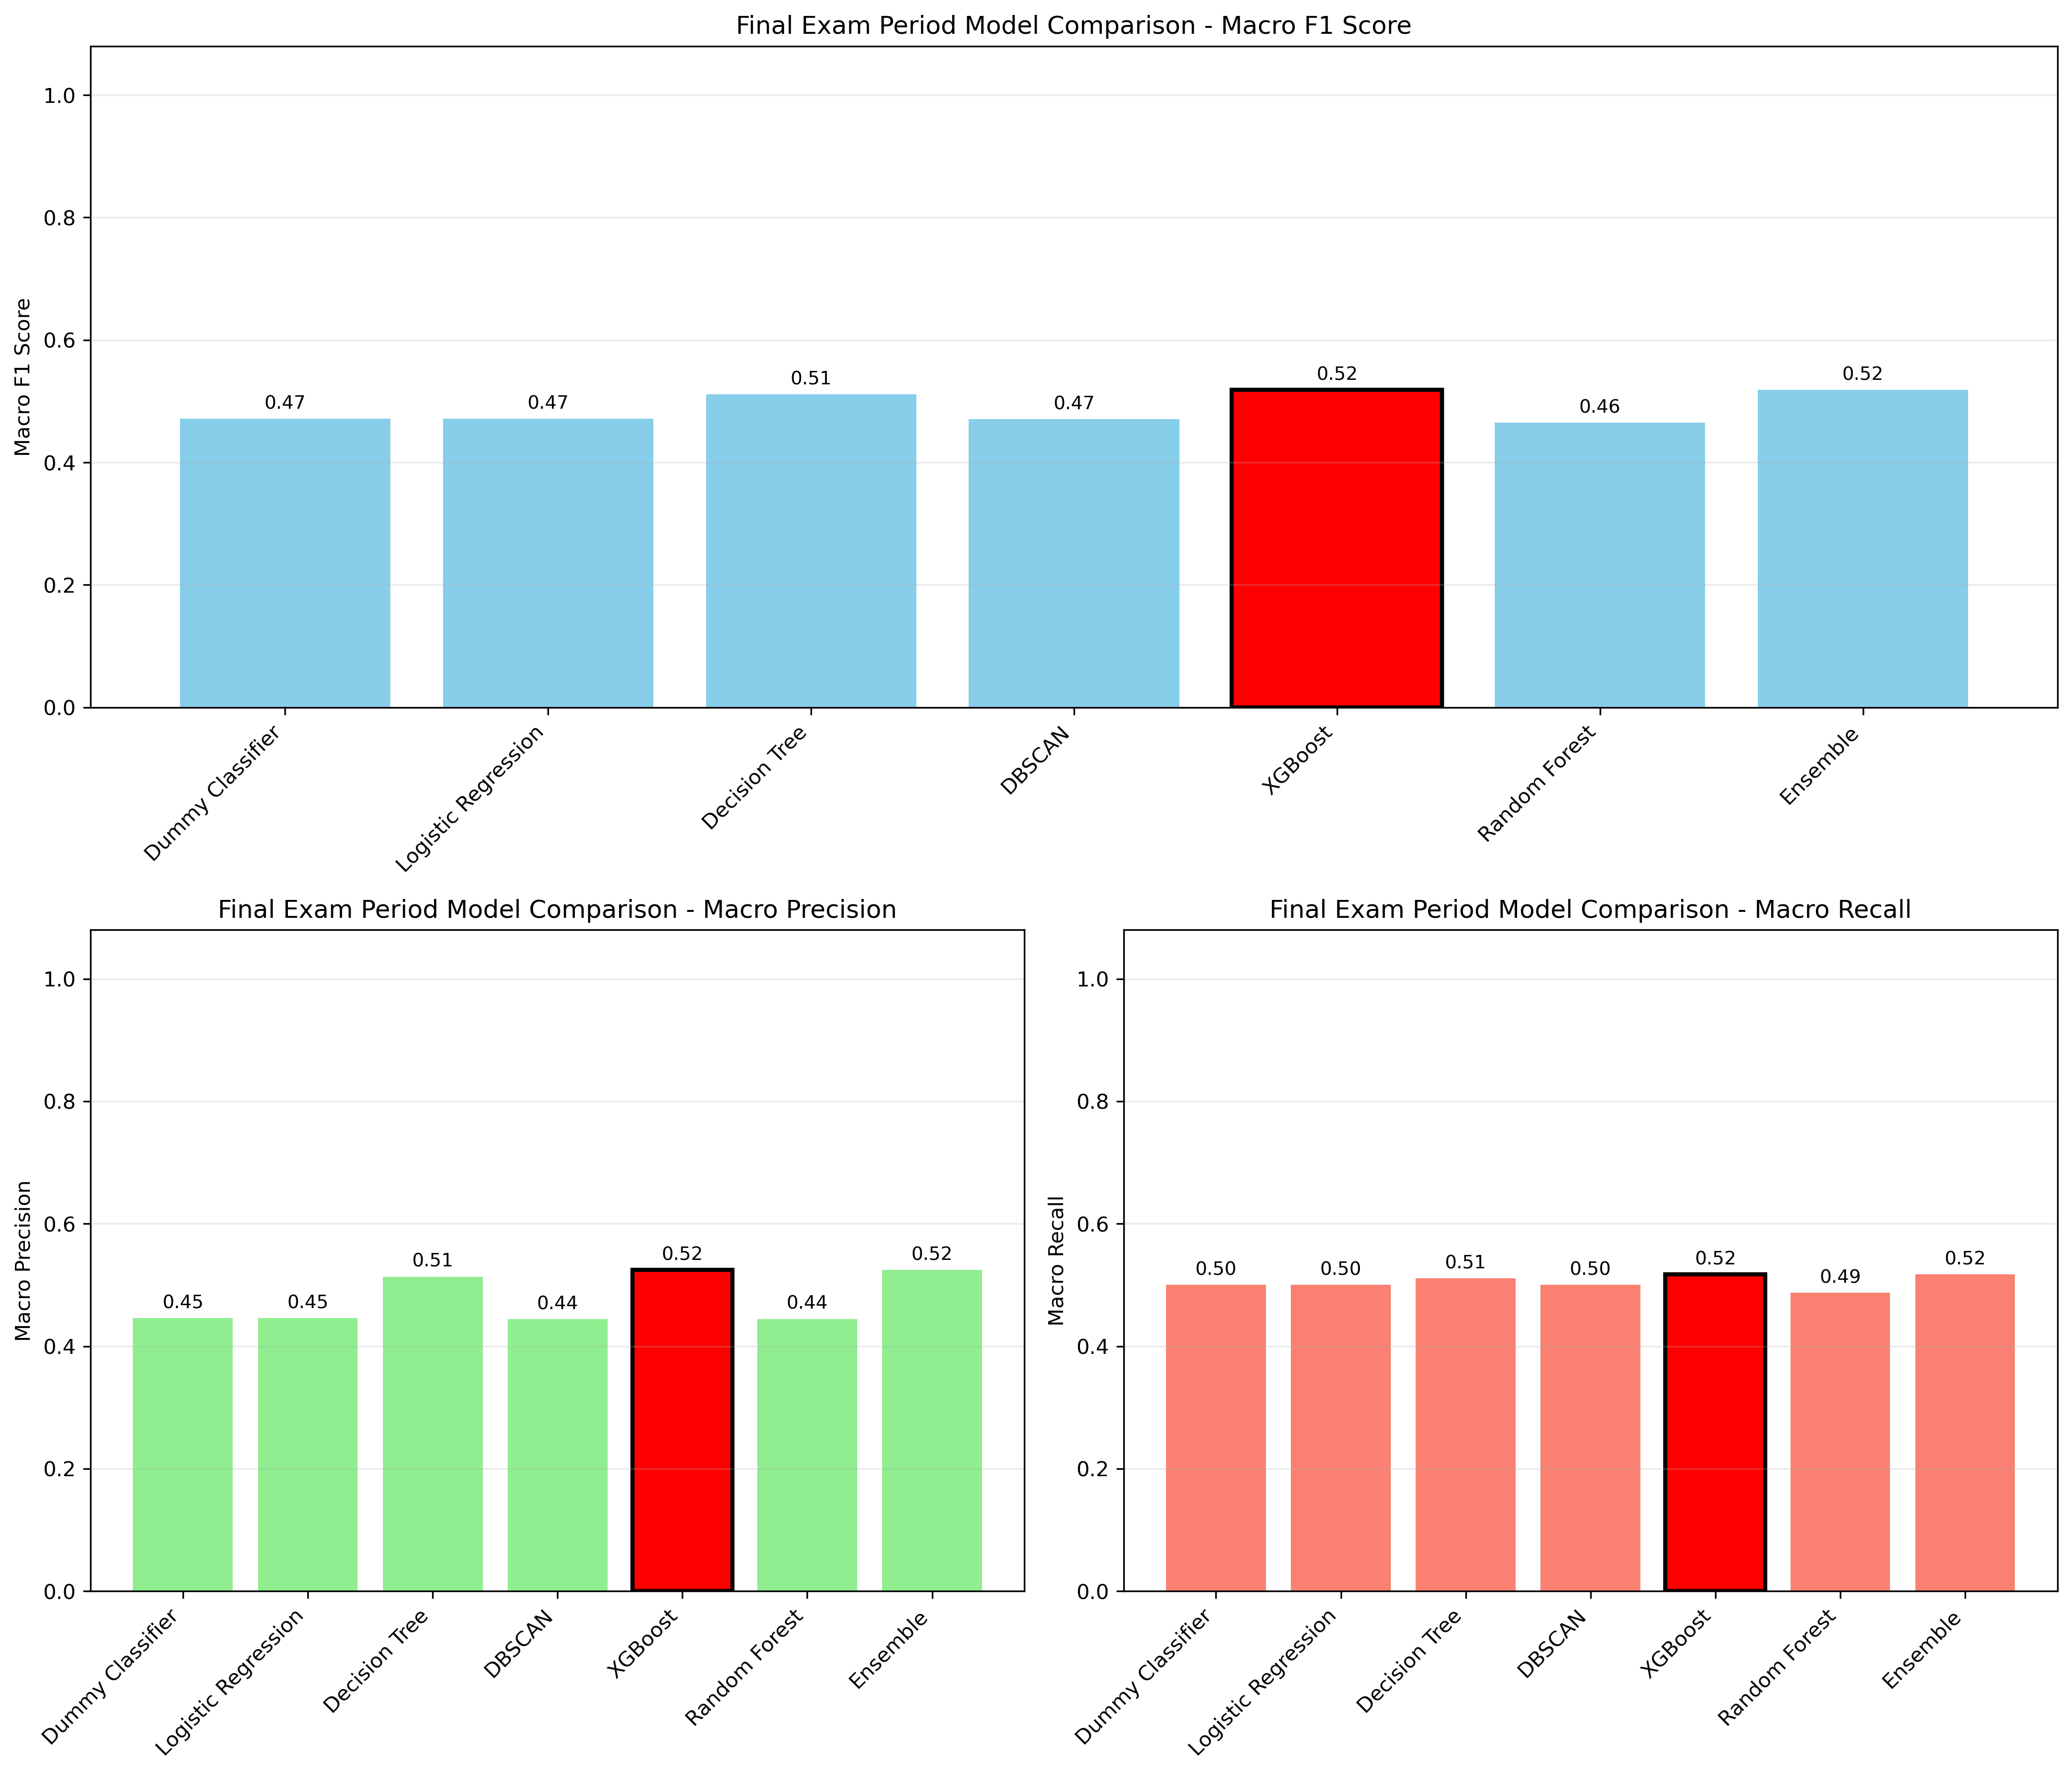
\includegraphics[width=0.88\textwidth]{../MachineLearning/results2/ACADEMICAL_PERIOD/Final_Model_Comparison_All_Metrics.png}
\caption{Final exam versus ordinary term model comparison.}
\label{fig:ml-final-comparison}
\end{figure}

\begin{figure}[H]
\centering
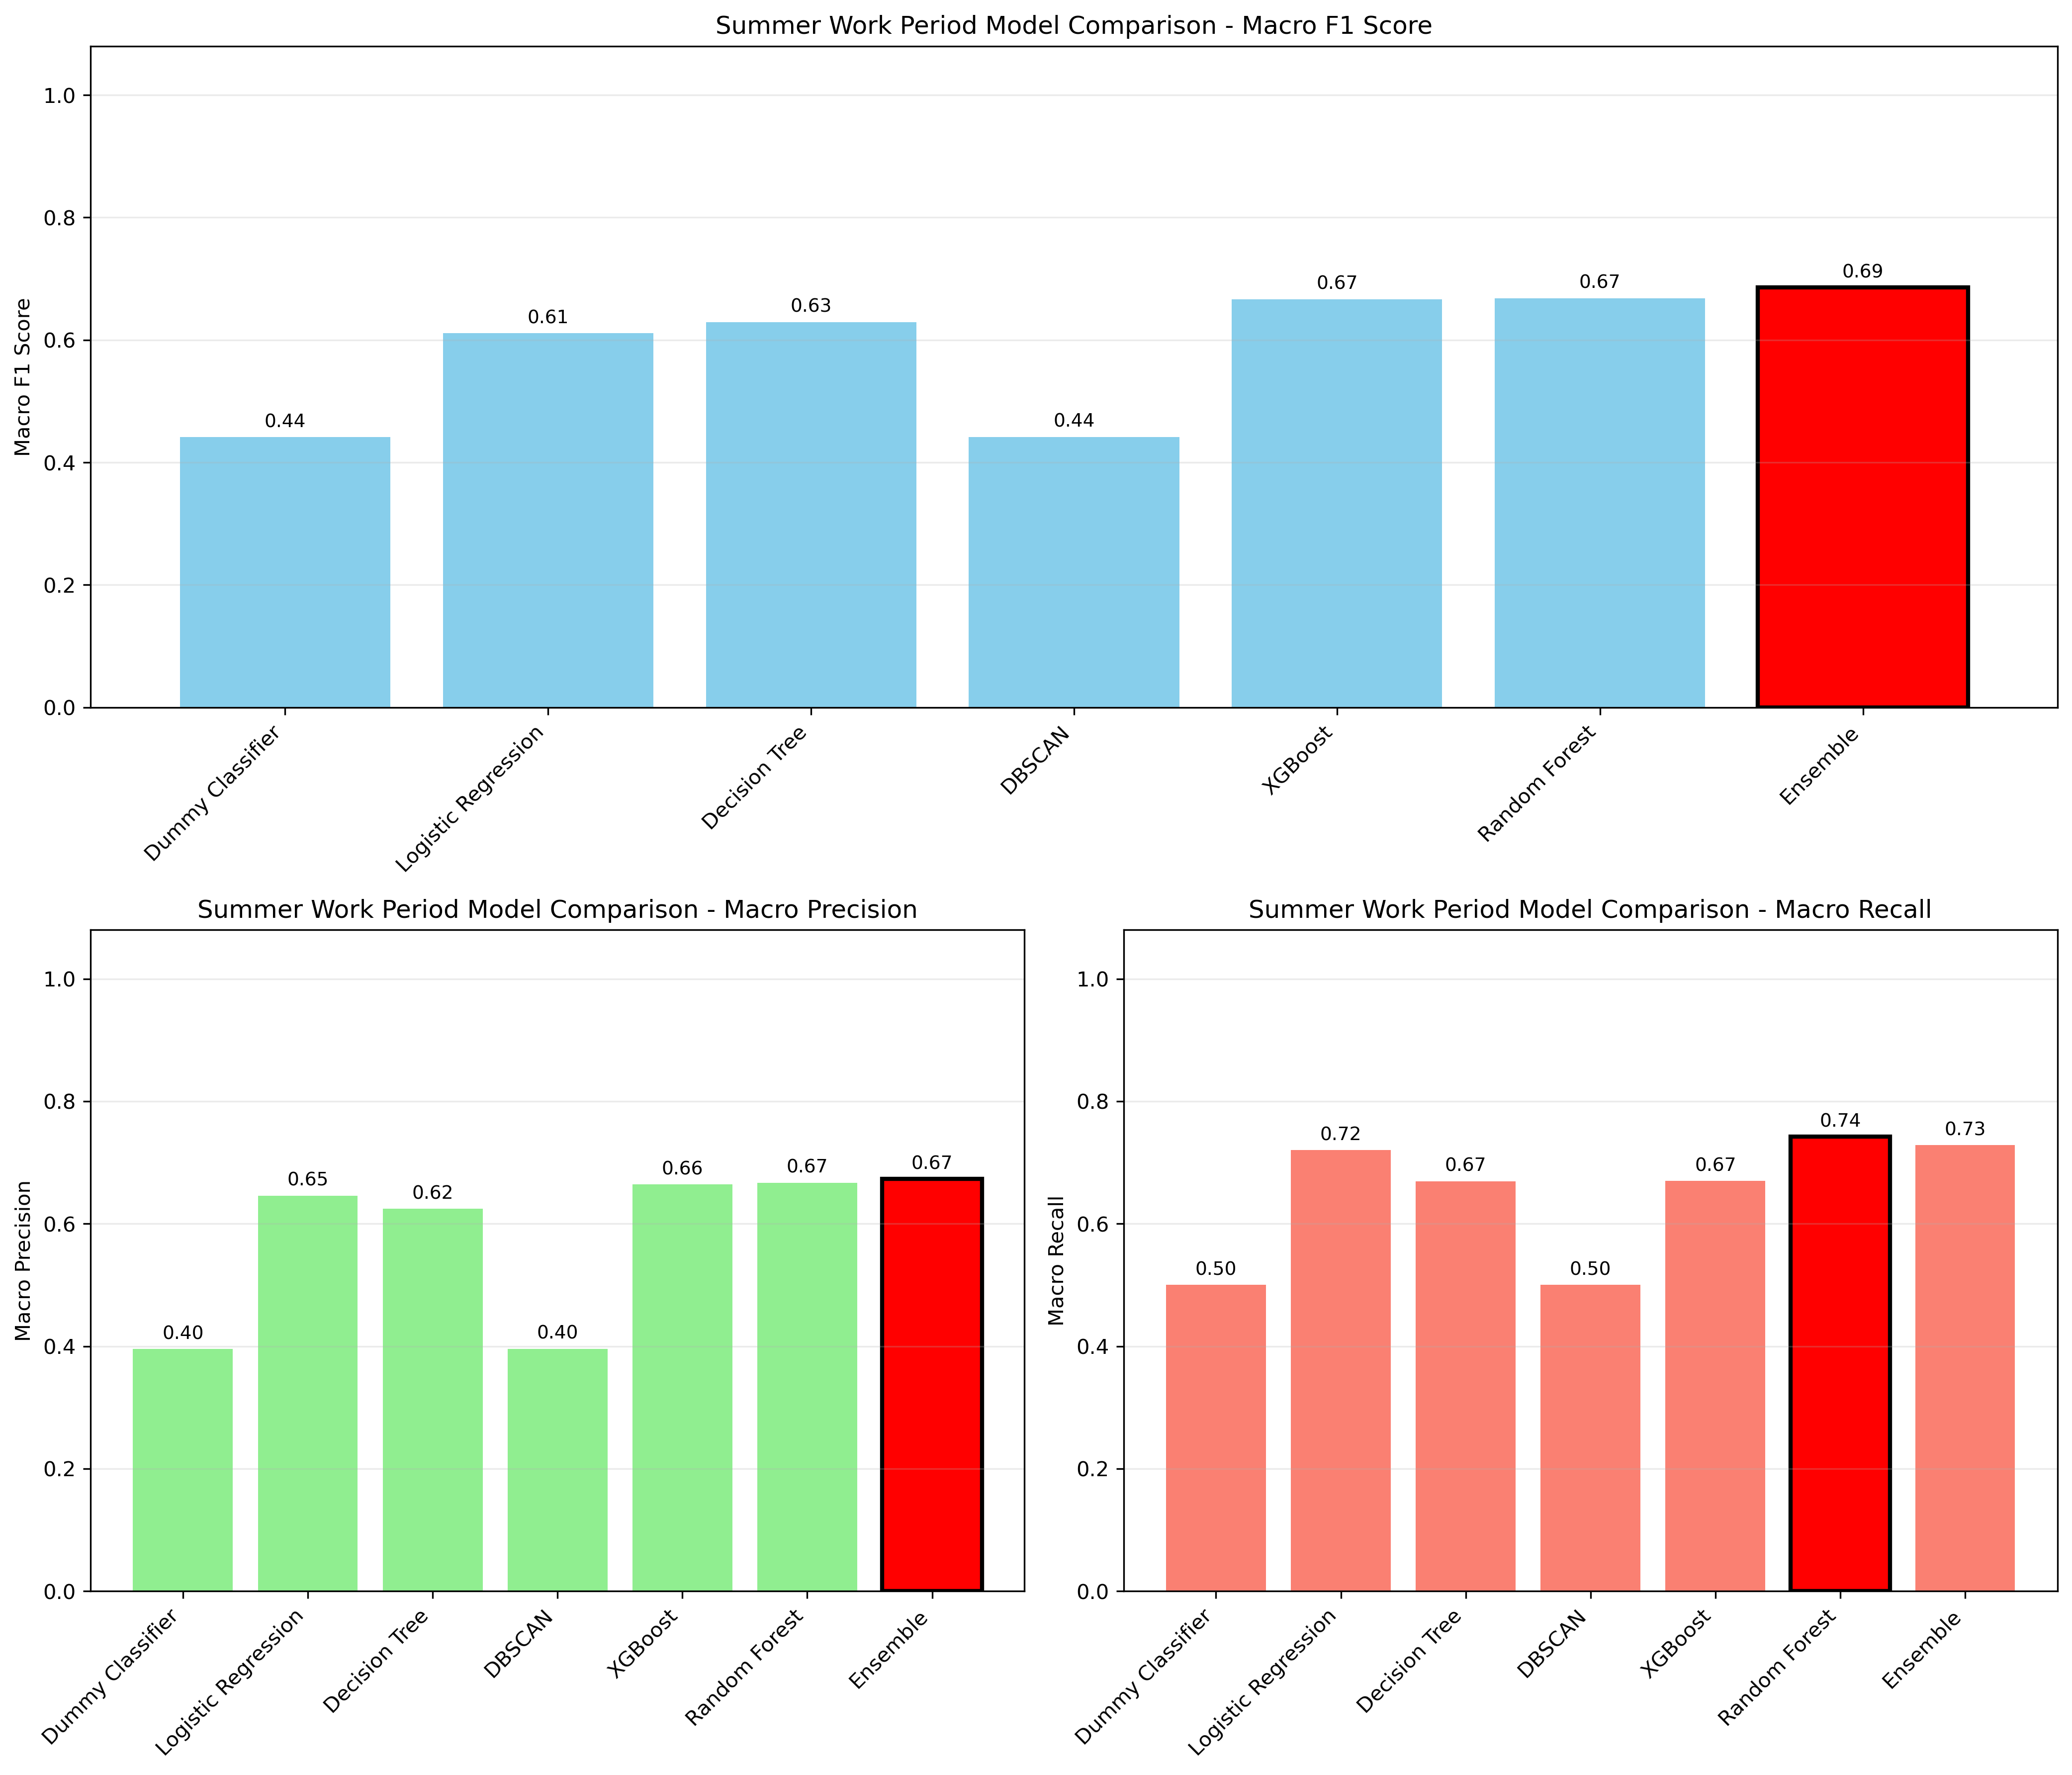
\includegraphics[width=0.88\textwidth]{../MachineLearning/results2/SUMMER_WORK_PERIOD/summer_model_comparison_all_metrics.png}
\caption{Summer work versus ordinary term model comparison.}
\label{fig:ml-summer-comparison}
\end{figure}

\begin{figure}[H]
\centering
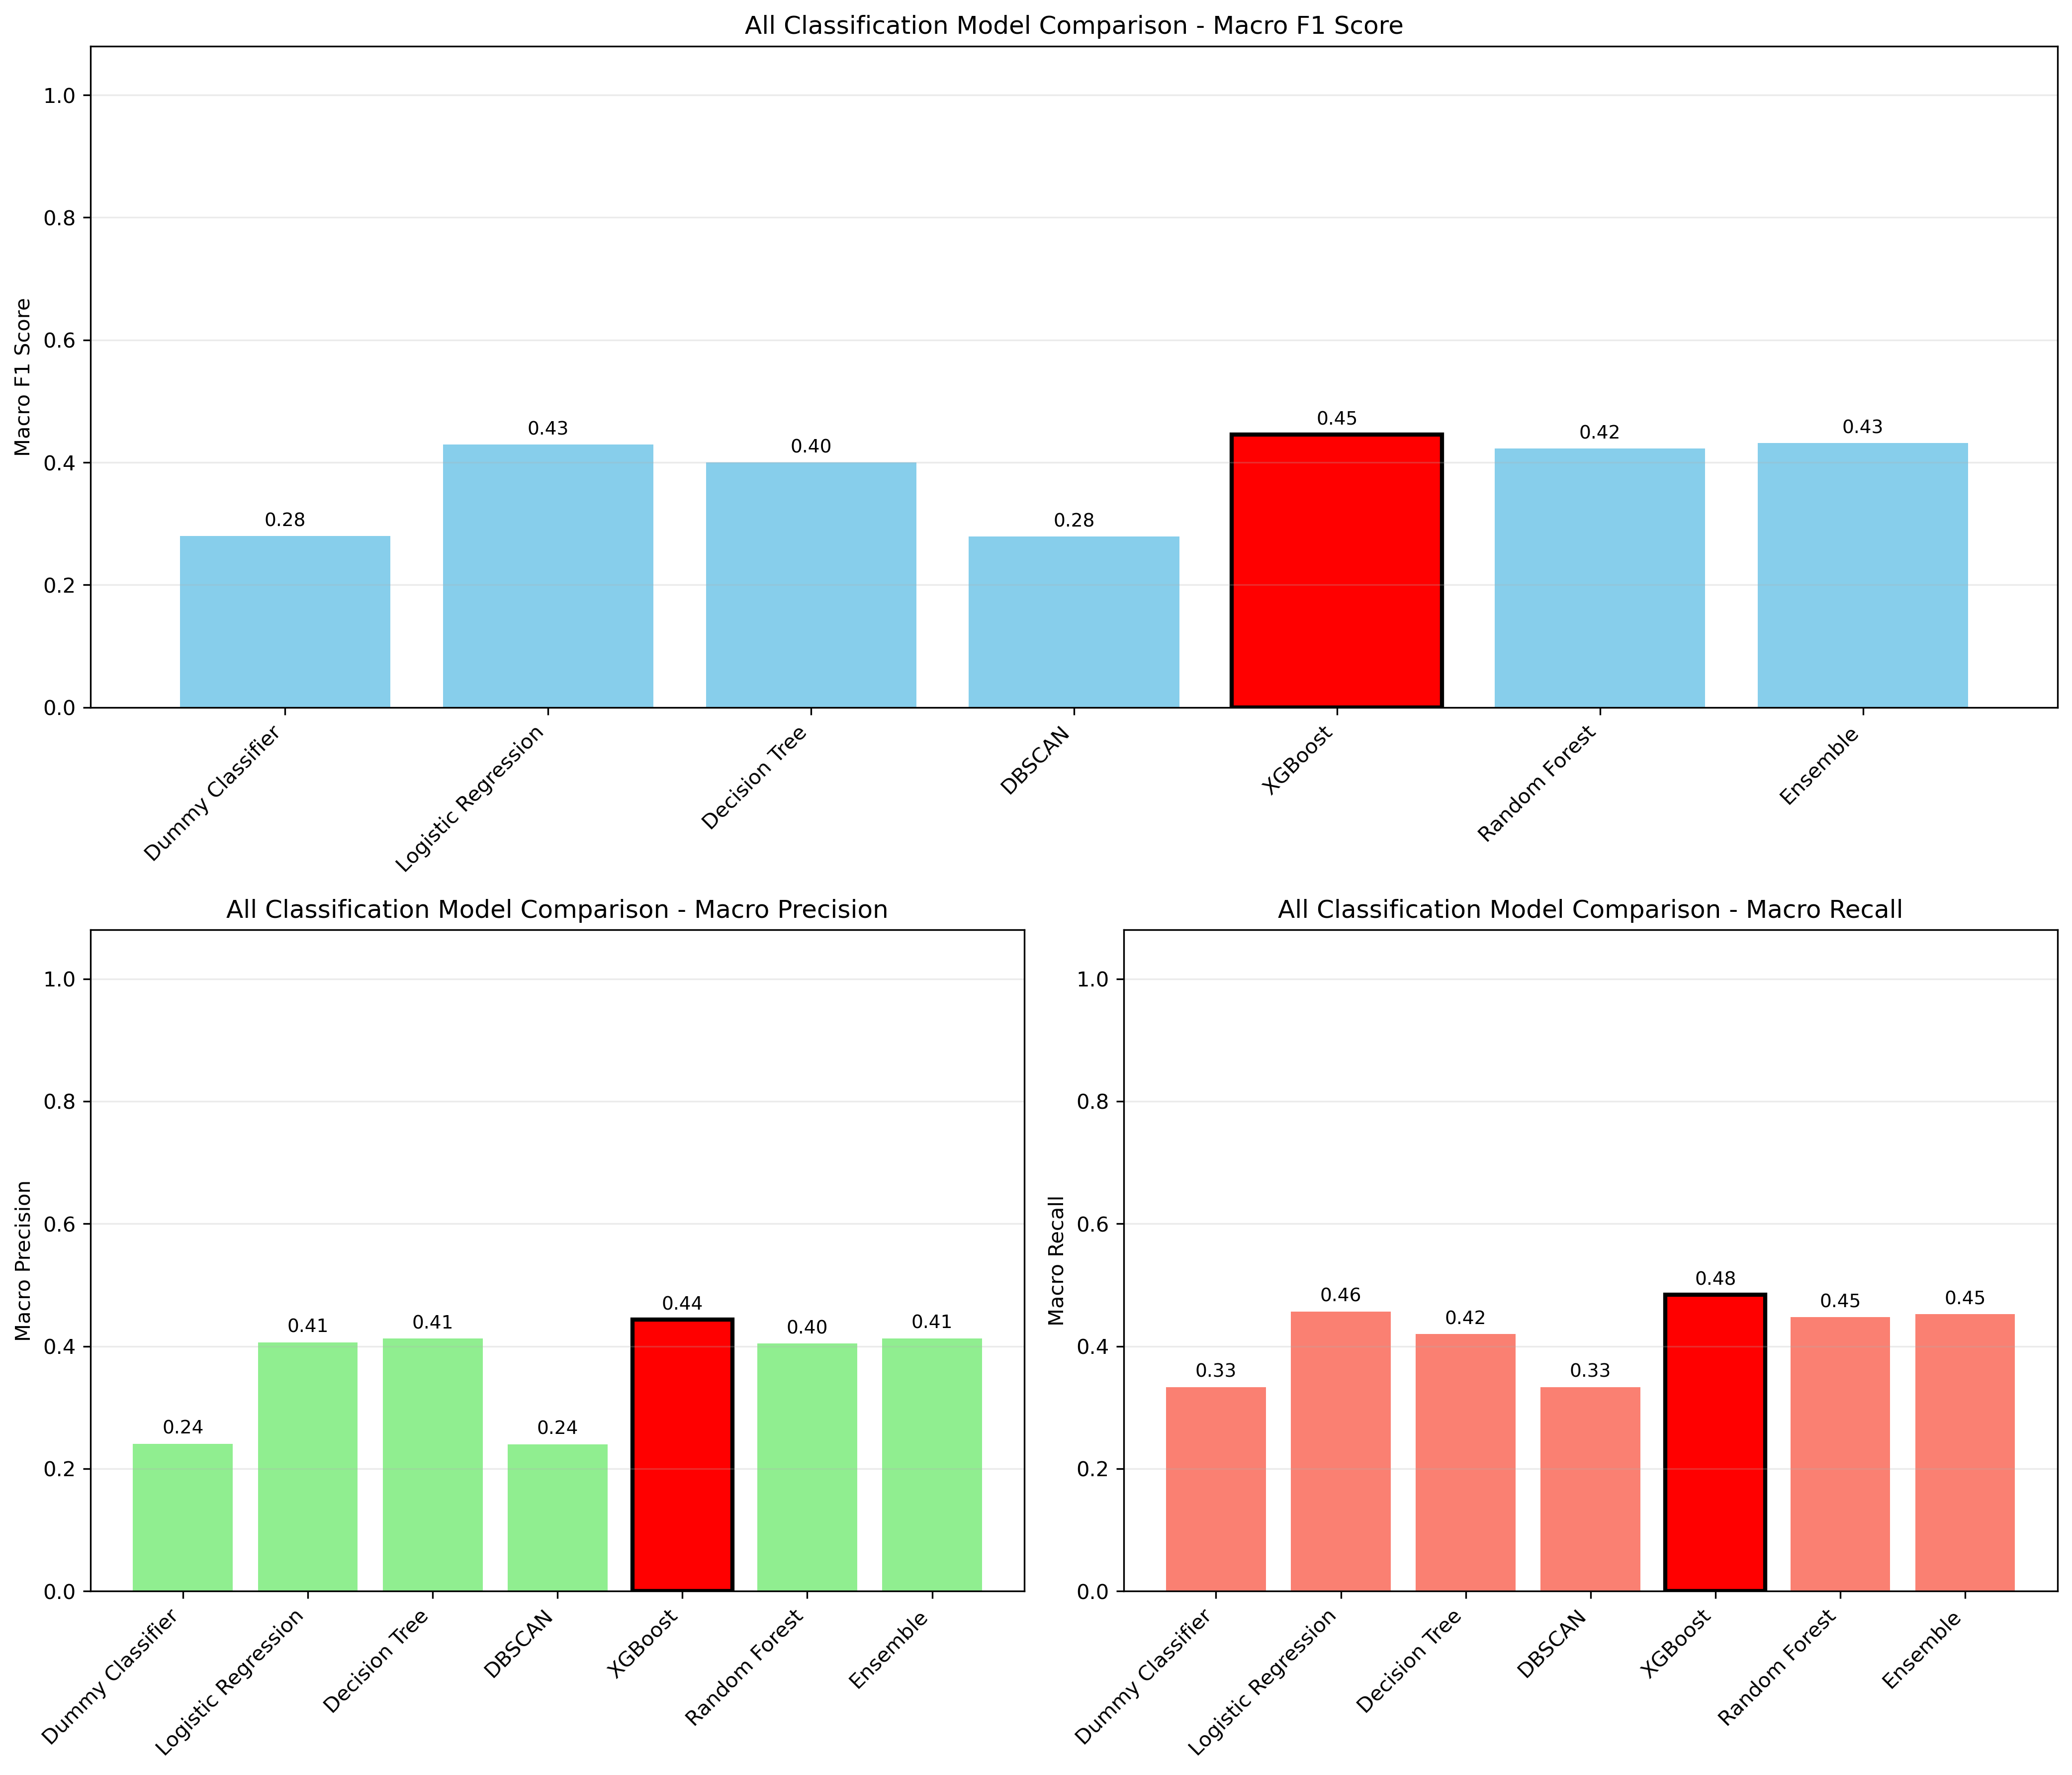
\includegraphics[width=0.88\textwidth]{../MachineLearning/results2/All_CLASSIFICATION/all_model_comparison_all_metrics.png}
\caption{All-period multiclass model comparison.}
\label{fig:ml-all-comparison}
\end{figure}

The confusion-matrix heatmaps below show the best-performing model for each task. For the final exam task, XGBoost and the ensemble tie in macro F1; I show XGBoost. For summer work, the ensemble is the strongest. For all-period classification, XGBoost is the strongest.

\begin{figure}[H]
\centering
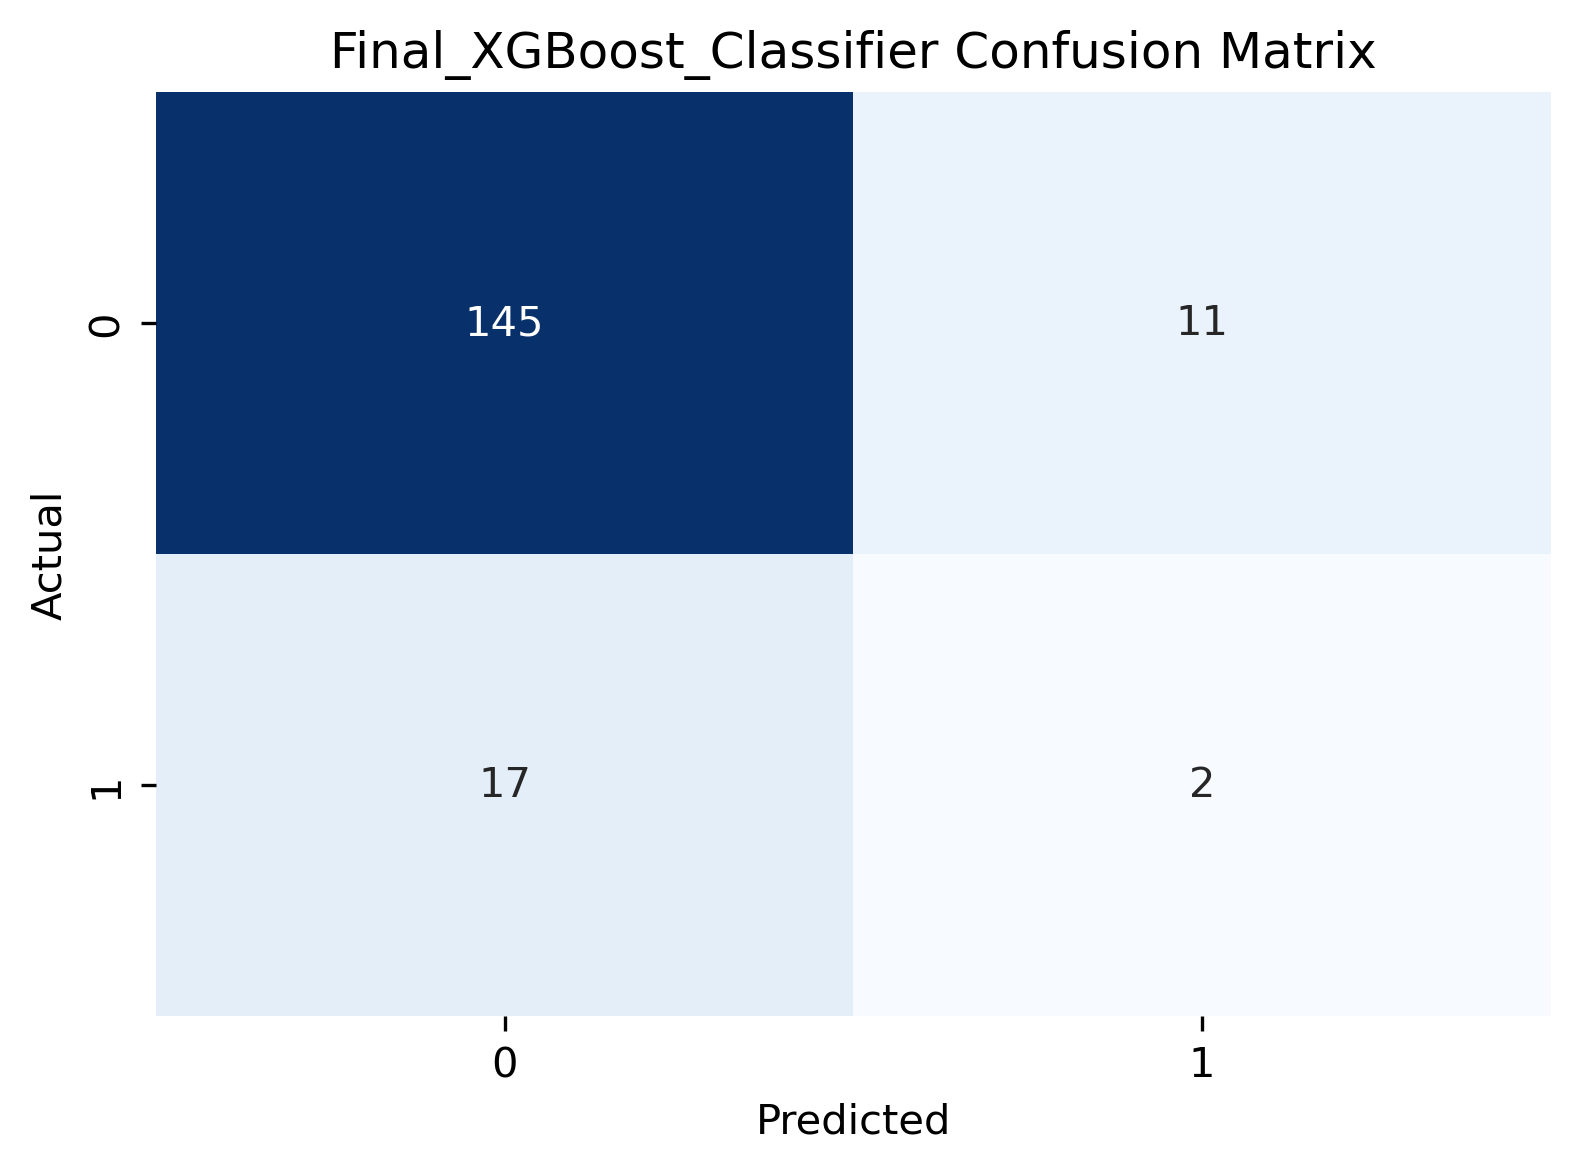
\includegraphics[width=0.68\textwidth]{../MachineLearning/results2/ACADEMICAL_PERIOD/Final_XGBoost_Classifier_confusion_matrix.png}
\caption{Final exam versus ordinary term heatmap for XGBoost.}
\label{fig:ml-final-heatmap}
\end{figure}

\begin{figure}[H]
\centering
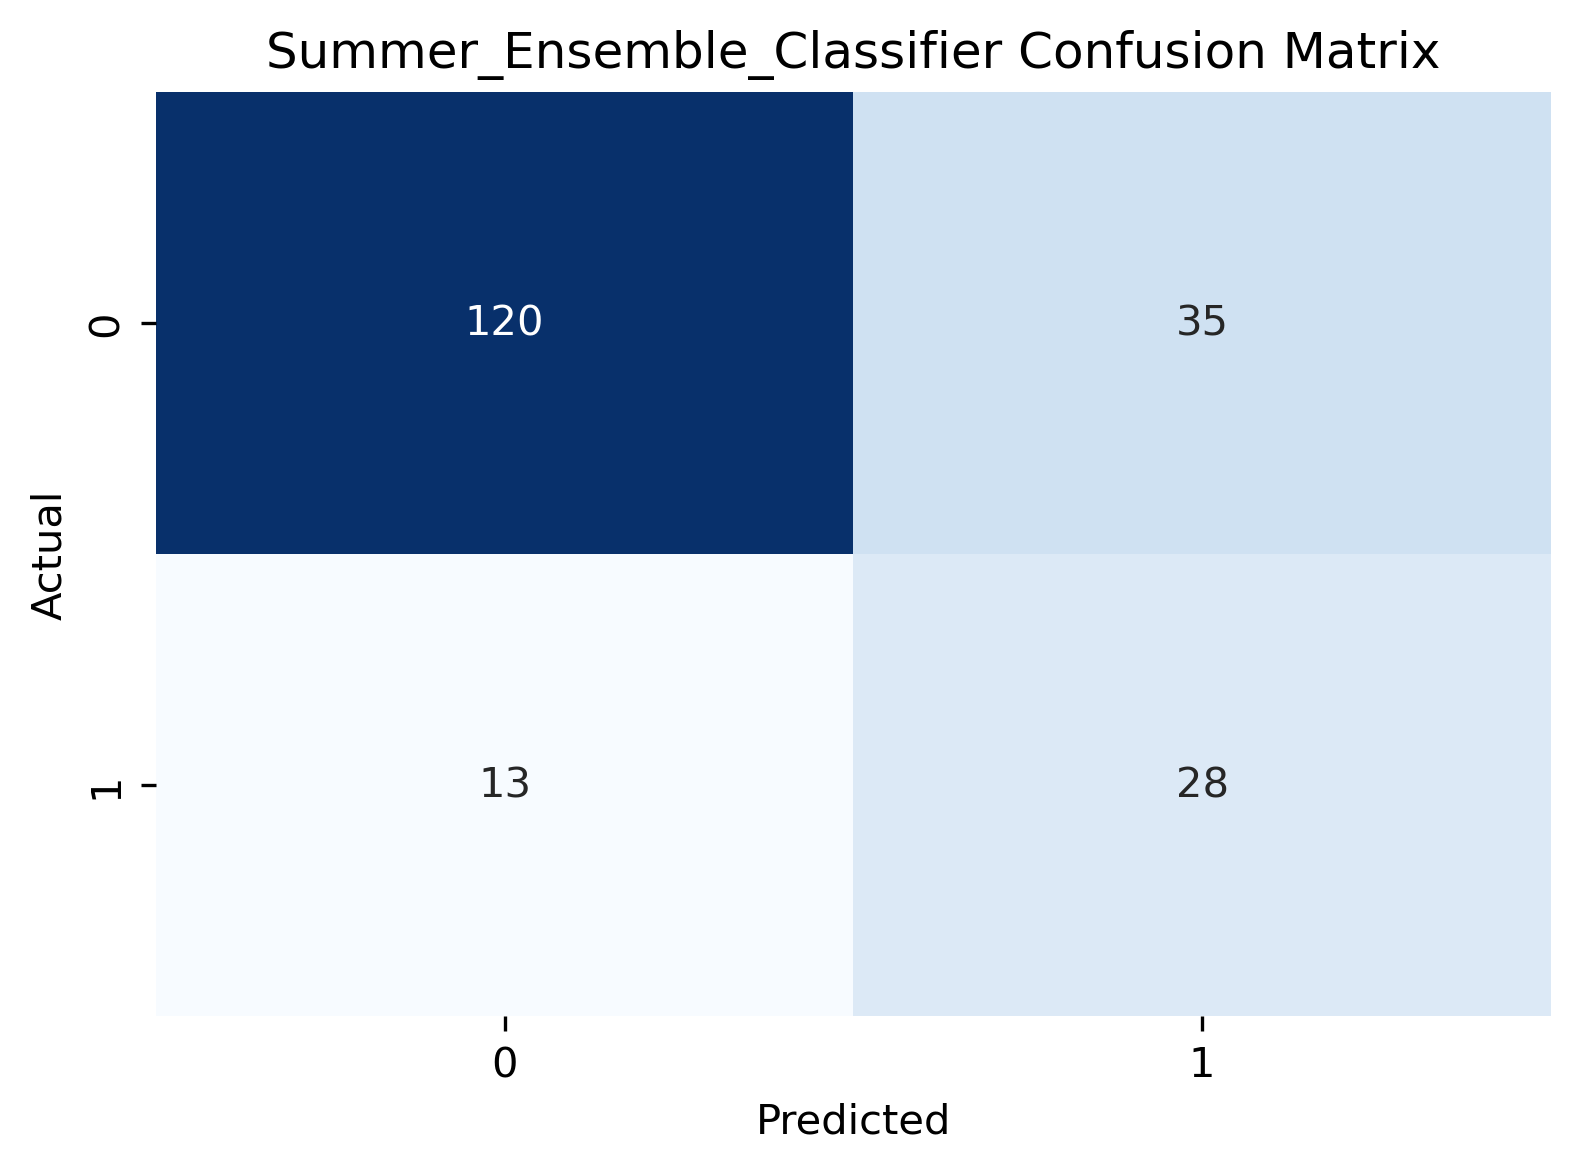
\includegraphics[width=0.68\textwidth]{../MachineLearning/results2/SUMMER_WORK_PERIOD/Summer_Ensemble_Classifier_confusion_matrix.png}
\caption{Summer work versus ordinary term heatmap for the ensemble model.}
\label{fig:ml-summer-heatmap}
\end{figure}

\begin{figure}[H]
\centering
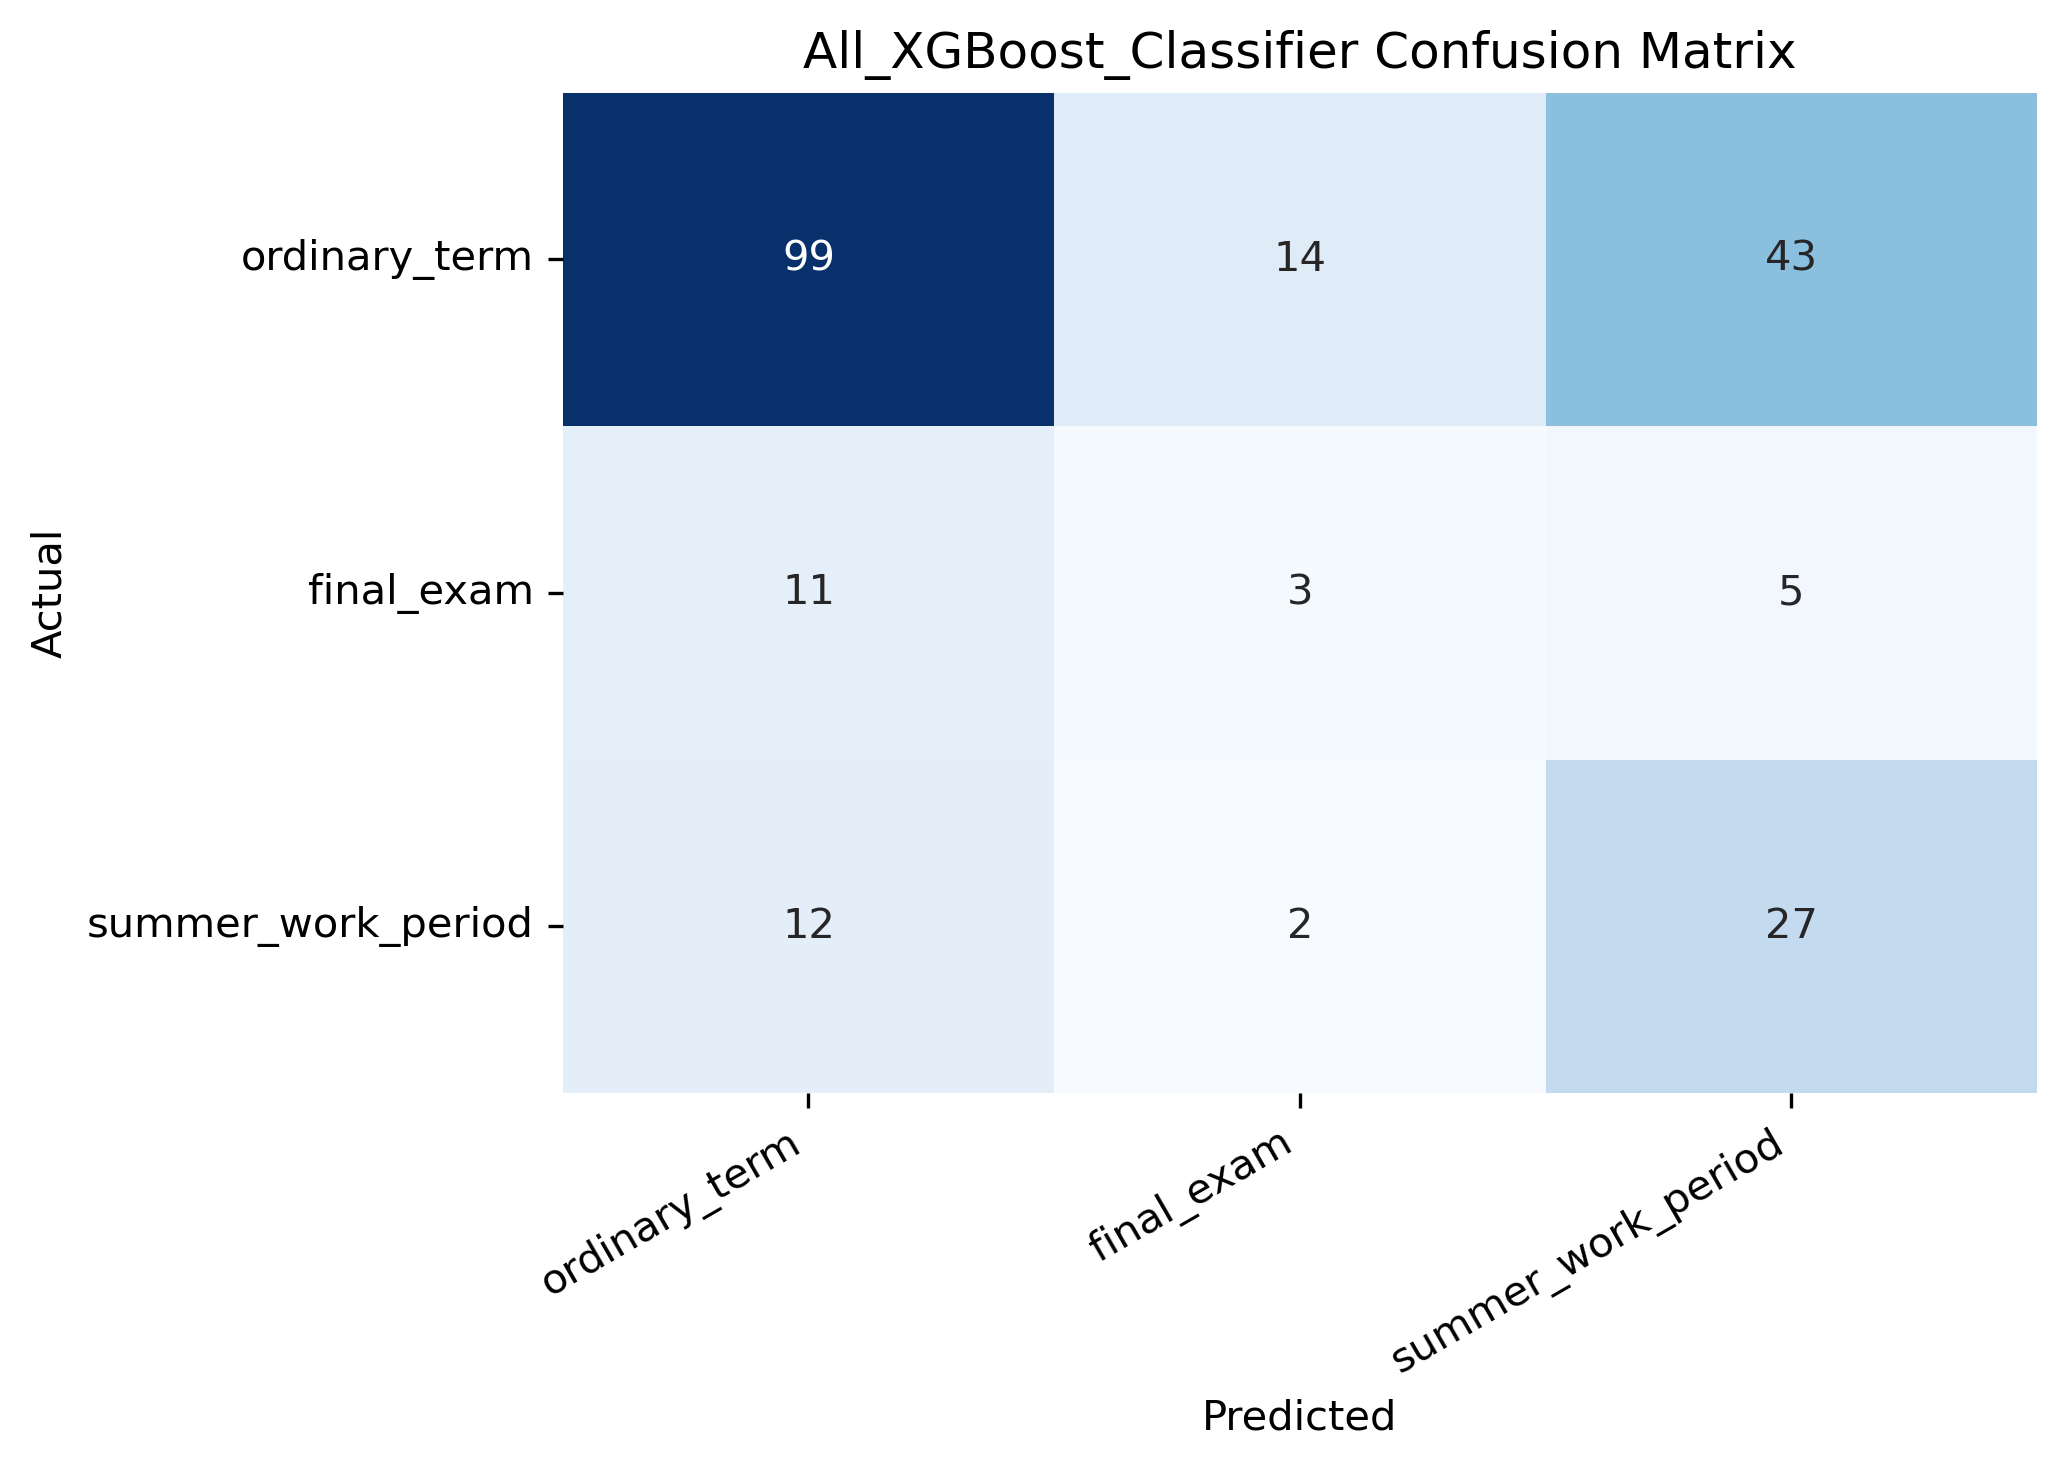
\includegraphics[width=0.72\textwidth]{../MachineLearning/results2/All_CLASSIFICATION/All_XGBoost_Classifier_confusion_matrix.png}
\caption{All-period multiclass heatmap for XGBoost.}
\label{fig:ml-all-heatmap}
\end{figure}

\section{Findings}

The EDA shows that the platforms have different behavioral structures. Spotify is the most continuous platform, while Netflix and Prime Video are much more sparse and bursty. YouTube has high variability and strong evening/night activity. Cross-platform correlations are generally limited, except for variables that belong to the same platform.

The hypothesis tests do not provide strong evidence that total entertainment usage is broadly lower during finals. The final-exam window is also only an imperfect proxy for academic pressure, because workload can vary by course and some stressful academic days may fall outside the formal final-exam period. The long-form streaming test also moved in the opposite direction from the alternative, because YouTube watched count was higher on Netflix + Prime active days on average. However, late-evening YouTube and Spotify shares are significantly lower during finals, suggesting that time-of-day behavior changes more clearly than total daily activity. The late-evening/time-of-day decomposition is one of the most original parts of the project because the significant effects appear there rather than in broad daily totals. Spotify and YouTube also have a statistically significant same-day association, but $\rho=0.0934$ is close to zero, so the relationship is very weak in practical terms.

The machine learning results suggest that summer work behavior is easier to classify within the current task-specific setup than final exam behavior. Final exam versus ordinary term classification improves only from 47.13\% dummy macro F1 to 51.85\% best macro F1. Summer work versus ordinary term improves from 44.16\% to 68.59\%. The all-period task improves from 27.96\% to 44.52\%. However, the summer task also uses two additional late-evening share features, so part of the stronger summer result may come from this richer feature set. Overall, the current task-specific entertainment features capture summer work patterns more clearly than final exam patterns, but the comparison is not fully apples-to-apples.

\section{Additional Presentation Material}

The project includes a public website built with Next.js and deployed on Vercel:

\begin{center}
\url{https://dsa-210-term-project-ten.vercel.app/}
\end{center}

The website presents the same project through interactive SVG charts, result cards, machine learning visualizations, and an appendix image gallery. It is used as additional presentation material alongside the notebooks, report, and public repository files.

\section{Limitations and Future Work}

There are several limitations. First, the datasets have different levels of temporal detail. YouTube and Spotify have timestamps, but Netflix and Prime Video are mostly date-level. Second, the data is personal and therefore does not generalize to other users. Third, long-form streaming is sparse, which makes some comparisons unstable. Fourth, the academic labels are coarse: midterms are not separately labeled, and final exam periods may not fully represent academic pressure.

For future work, additional behavioral sources such as ChatGPT usage, social-media usage, or calendar workload could be added if privacy can be handled carefully. Instagram is especially important because it can take a significant amount of time through what is often described as ``scrolling endlessly.'' Therefore, its absence may reduce classification quality because an important entertainment-related behavior is missing from the feature set.

Time-series features such as lagged activity, rolling averages, and previous-day behavior could also improve the machine learning models. In this version, days are treated as different samples; however, nearby days may still be related. For example, a very large amount of entertainment activity on consecutive days might suggest an ordinary-term pattern rather than a final-exam pattern. Finally, the machine learning part could be improved with a more time-aware validation strategy because behavior across nearby days is not fully independent.

\section{Conclusion}

This project shows that my entertainment behavior can be studied meaningfully through personal platform exports when privacy and cleaning decisions are handled carefully. The strongest statistical evidence in my data appears in late-evening activity changes rather than total platform usage. The machine learning results show that the current task-specific features capture my summer work behavior better than my final exam behavior, while the different feature sets mean this comparison should be interpreted cautiously. Overall, the project supports the idea that academic and work periods leave some signal in my personal entertainment patterns, but the signal is uneven and depends strongly on the period being classified.

\clearpage
\appendix
\section{Appendix: Additional Figures}

This appendix includes supporting figures that are useful for traceability but are not all discussed in detail in the main body.

\subsection{Additional EDA Figures}

\appendixfig{0.82}{../EDA/youtube_images/youtube_activity_count_by_action.png}{YouTube activity by action.}
\appendixfig{0.82}{../EDA/youtube_images/youtube_activity_count_by_hour.png}{YouTube activity by hour.}
\appendixfig{0.82}{../EDA/youtube_images/youtube_monthly_watched_and_search_counts.png}{Monthly YouTube watched and search counts.}
\appendixfig{0.82}{../EDA/spotify_images/spotify_monthly_listening_hours.png}{Monthly Spotify listening hours.}
\appendixfig{0.82}{../EDA/spotify_images/spotify_daily_streams_vs_hours.png}{Daily Spotify streams versus listening hours.}
\appendixfig{0.82}{../EDA/spotify_images/spotify_listening_hours_by_hour.png}{Spotify listening by hour.}
\appendixfig{0.82}{../EDA/prime_netflix_images/total_long_form_count_by_platform_common_range.png}{Total long-form count by platform.}
\appendixfig{0.82}{../EDA/prime_netflix_images/monthly_combined_long_form_count.png}{Monthly combined long-form streaming count.}
\appendixfig{0.82}{../EDA/combined_images/combined_platform_activity_by_analysis_period_boxplots.png}{Platform activity by academic period.}
\appendixfig{0.82}{../EDA/combined_images/combined_relative_activity_by_analysis_period.png}{Relative activity by academic period.}
\appendixfig{0.82}{../EDA/combined_images/combined_platform_diversity_by_analysis_period.png}{Platform diversity by academic period.}
\appendixfig{0.82}{../EDA/combined_images/combined_spotify_hours_vs_youtube_watched_scatter.png}{Spotify hours versus YouTube watched count.}
\appendixfig{0.82}{../EDA/combined_images/combined_netflix_prime_vs_youtube_watched_scatter.png}{Netflix plus Prime count versus YouTube watched count.}

\subsection{Additional Machine Learning Figures}

\appendixfig{0.7}{../MachineLearning/results2/ACADEMICAL_PERIOD/Final_Decision_Tree_Visualization.png}{Final-exam decision tree visualization.}
\appendixfig{0.7}{../MachineLearning/results2/SUMMER_WORK_PERIOD/Summer_Decision_Tree_Visualization.png}{Summer-work decision tree visualization.}
\appendixfig{0.7}{../MachineLearning/results2/All_CLASSIFICATION/All_Decision_Tree_Visualization.png}{All-period decision tree visualization.}
\appendixfig{0.7}{../MachineLearning/results2/ACADEMICAL_PERIOD/Final_DBSCAN_Cluster_Map.png}{Final-exam DBSCAN cluster map.}
\appendixfig{0.7}{../MachineLearning/results2/All_CLASSIFICATION/All_DBSCAN_PCA_Visualization.png}{All-period DBSCAN PCA visualization.}
\appendixfig{0.7}{../MachineLearning/results2/ACADEMICAL_PERIOD/Final_Model_Comparison_F1_Score.png}{Final-exam macro F1 comparison.}
\appendixfig{0.7}{../MachineLearning/results2/SUMMER_WORK_PERIOD/summer_model_comparison_f1_score.png}{Summer-work macro F1 comparison.}

\section{AI Assistance Disclosure}

AI assistance was used for debugging code, organizing report structure, writing LaTeX scaffolding, and checking consistency between the notebook outputs, README, and website text. The data sources, analysis goals, and project decisions are my own.

\end{document}
